\documentclass[11pt,a4paper]{article}
\usepackage[utf8]{inputenc}
\usepackage[T1]{fontenc}
\usepackage{lmodern}
\usepackage[spanish,es-noquoting,es-nodecimaldot,es-tabla]{babel}
\usepackage[a4paper,margin=2.1cm,top=2.2cm,bottom=2.3cm]{geometry}
\usepackage{amsmath,amssymb}
\usepackage{graphicx}
\usepackage{booktabs,tabularx,longtable,multirow,array}
\usepackage[table]{xcolor}
\usepackage{float}
\usepackage{caption}
\usepackage{enumitem}
\usepackage{fancyhdr}
\usepackage{pdflscape}
\usepackage{tcolorbox}
\usepackage{microtype}
\usepackage[hidelinks]{hyperref}

\definecolor{azul}{HTML}{1F4E9C}
\definecolor{gris}{HTML}{404040}
\newtcolorbox{idea}[1][]{colback=azul!5,colframe=azul!60,boxrule=0.6pt,arc=2pt,left=6pt,right=6pt,top=4pt,bottom=4pt,#1}
\newtcolorbox{ojo}[1][]{colback=orange!6,colframe=orange!70!black,boxrule=0.6pt,arc=2pt,left=6pt,right=6pt,top=4pt,bottom=4pt,#1}
\newcommand{\sig}[1]{\texttt{\color{azul}#1}}
\newcommand{\bus}[1]{\texttt{#1}}
\setlength{\parskip}{4pt}
\setlength{\parindent}{0pt}
\renewcommand{\arraystretch}{1.18}
\captionsetup{font=small,labelfont=bf}
\setlist{itemsep=2pt,topsep=3pt}

\pagestyle{fancy}
\fancyhf{}
\lhead{\small Proyecto \#8 · Image Processor (2D filters) · arquitectura v4.1}
\rhead{\small \thepage}
\lfoot{\footnotesize Edison Torres · Juan Guaman · Electrónica Digital}
\rfoot{\footnotesize 19 de noviembre de 2026}

\begin{document}

\begin{center}
{\LARGE\bfseries Image Processor (2D filters)}\\[4pt]
{\Large Arquitectura v4.1: esquemático simplificado y funcionamiento bloque por bloque}\\[8pt]
{\normalsize Edison Torres · Juan Guaman — Electrónica Digital, Escuela Colombiana de Ingeniería}\\
{\normalsize Nexys A7-100T (XC7A100T) · reloj de 100\,MHz · UART 115\,200\,Bd 8N1 · imagen 128\,×\,128 RGB}
\end{center}

\begin{idea}
\textbf{Qué se hizo, en seis líneas.}
(1) Se rediseñó toda la arquitectura para que tenga \emph{menos hardware sin perder ninguna función}: ahora se procesa un byte (un canal de color) a la vez, con un único camino de datos de 8\,bits.
(2) Se dibujó el esquemático en \textbf{una sola hoja A1} donde \emph{cada conexión es un cable dibujado}: no hay etiquetas o pestañas que entran y salen; solo los pines de la FPGA son pentágonos.
(3) Se reescribió el RTL en SystemVerilog (10 archivos, uno por bloque) con los mismos nombres de señales del esquemático.
(4) Se verificó con 10 testbenches autoverificables, todos en \textbf{PASS}, incluida la imagen completa de 128\,×\,128 en los cinco modos y con ruido, comparada byte a byte contra un modelo de referencia.
(5) Se llevó a \textbf{Vivado 2025.2} (simulación en xsim, síntesis, implementación y bitstream). La v4 \emph{no} cumplía los tiempos a 100\,MHz; la \textbf{v4.1} agrega un registro de segmentación en el MAC (REG\_PIX y REG\_W) y ahora cumple con 2,11\,ns de margen (sección~\ref{sec:tiempos}).
(6) Este documento explica cada bloque, cómo funciona el sistema completo, los anchos de bus y las decisiones con sus alternativas.
\end{idea}

\tableofcontents
\clearpage

% =====================================================================
\section{Qué cambió respecto a la versión v3 y por qué}

La versión v3 (ver \texttt{docs/03\_decisiones.md}) procesaba un píxel completo de 24\,bits por vez, con tres carriles idénticos (R, G y B), un carril aparte para el Unsharp, un multiplexor de salida de 24\,bits, un ensamblador de píxeles y un multiplexor de bytes para la transmisión. En total tenía 15 tipos de multiplexor (M1–M15) y 27 instancias. La v4 parte de una observación: \textbf{la UART es el cuello de botella}. Transmitir la imagen tarda 4,27\,s; calcular toda la imagen tarda unos pocos milisegundos. Hacer el cálculo más rápido no se nota; hacerlo más simple sí se nota en el esquemático, en la verificación y en la sustentación.

\begin{center}
\small
\begin{tabularx}{\linewidth}{>{\raggedright\arraybackslash}p{2.7cm}>{\raggedright\arraybackslash}X>{\raggedright\arraybackslash}X>{\raggedright\arraybackslash}p{1.6cm}}
\toprule
\textbf{Tema} & \textbf{v3 (antes)} & \textbf{v4 (ahora) y por qué} & \textbf{Req.} \\
\midrule
Ancho del camino de datos & 3 carriles de 8\,b en paralelo (píxel de 24\,b), SR\_PIX de 16\,b, TX\_BYTE y M14 para sacar los 3 bytes & \textbf{1 carril de 8\,b}: se calcula un canal por vez, en el mismo orden en que llegan y salen los bytes por la UART. Desaparecen el ensamblador, el contador TX\_BYTE, M14 y dos carriles completos. Costo: el cálculo pasa de $\approx$1,8\,ms a 5,9\,ms por pasada en v4.1 (invisible frente a 4,27\,s de UART). & R-P1, R-P2 \\
Memorias & 2 × 16\,384 × 24\,b & 2 × 65\,536 × 8\,b con dirección \{fila, columna, canal\}. El vecino se obtiene sumando $\pm1$ a fila y columna; no hace falta multiplicar por 3. Se desperdicia el 25\,\% (canal 3) pero sobra BRAM. & R-P1 \\
Unsharp & Carril aparte: $d = 2I - G$, M11 y M12 & \textbf{Un kernel más en la ROM}: $2I - G/16 = \tfrac{1}{16}(32\,\delta - G) * I$. Sale con el mismo hardware que los demás filtros. & R-P1 \\
Bypass & Entrada propia en M13 & \textbf{Kernel identidad} ($16\,\delta$) en la ROM: no hay multiplexor de salida. & R-G04 \\
Pesos y normalización & Pesos por desplazamiento (M7: 0/×1/×2/×4 y signo), ACC de 13\,b, M8–M10 por carril & \textbf{Multiplicador 9\,×\,8 con signo} (presentación 7, diapositivas 84–86), con un registro de segmentación delante desde v4.1, y todos los kernels multiplicados por 16: la normalización es siempre $\div 16$, que son \emph{solo cables}. & R-P1 \\
Contadores de posición & WR\_CNT y BYTE\_CNT para recibir; COL\_CNT y ROW\_CNT para procesar & \textbf{Un solo contador \{ROW, COL, CH\}} compartido: en IDLE avanza con cada byte recibido y en P1/P2 con cada byte calculado. & R-P2 \\
Bordes & M4 y M5 con sumas de 9\,b y comparaciones & \textbf{Sumador de 8\,b + MUX}: el bit más significativo de la suma dice si el vecino se sale (ver bloque 5). & R-P1 \\
Receptor UART & FSM de 4 estados & \textbf{Sin FSM}: un flip-flop RX\_BUSY y dos contadores. & R-P2 \\
Transmisor UART & M15 a la salida & La línea es directamente \bus{SR\_TX[0]}; el registro se rellena con unos, así queda en reposo sin multiplexor. & R-P2 \\
Ruido & M1 (umbral 0/8/16/32), M2 y M3 de 24\,b & Umbral $=$ \bus{SW[4:3]}$\times16$ (shifter, solo cables), valor $=$ \{8\{\bus{lfsr[8]}\}\} (cables) y un MUX de 8\,b. LFSR libre que se congela durante los 3 bytes de cada píxel. & R-P4 \\
Esquemático & Pestañas (etiquetas) que entran y salen & \textbf{Cables dibujados de origen a destino}, puntos en las uniones y saltos en los cruces sin conexión. & R-G06 \\
\bottomrule
\end{tabularx}
\end{center}

\textbf{Qué se mantiene igual (decisiones vigentes):} bordes replicados (D1), Laplaciano y LoG con valor absoluto saturado a 255 (D2), Unsharp con $k = 1$ (D3), ruido generado en la FPGA (D4), estilo SystemVerilog de las presentaciones 4 y 8 (D11), parámetros para simular rápido (D14), sin sincronizadores ni antirrebote (D15, D16), sin cabecera ni timeout (D17), sin estado de envío ni BRAM de salida (D18), la ROM de pesos ``corrida un tap'' (D19), el LoG en dos pasadas y el mismo protocolo con el PC: 49\,152 bytes de ida y 49\,152 de vuelta.

\textbf{Resultado:} 8 multiplexores dibujados (MUX\_BUSY, MUX\_RUIDO, MUX\_SRC, MUX\_ROW, MUX\_COL, MUX\_A, MUX\_B y MUX\_SAT) en lugar de 27 instancias. En Vivado 2025.2, la v4.1 implementada usa \textbf{313 LUT, 137 flip-flops, 32 bloques RAMB36} (23,7\,\% de los 135 que el reporte da para el XC7A100T), \textbf{0 DSP} y 18 pines, y \textbf{cumple los tiempos a 100\,MHz} con WNS $= +2{,}112$\,ns.

\begin{ojo}
\textbf{Diferencias de comportamiento que deben conocer (todas pequeñas):}
\begin{itemize}
\item Densidades de ruido: ahora 0\,\%, 6,25\,\%, 12,5\,\% y 18,75\,\% (antes 0, 3,1, 6,25 y 12,5\,\%). Siguen siendo 4 niveles con \bus{SW[4:3]}.
\item El patrón de ruido cambia en cada envío, porque el LFSR corre libre mientras espera (explicado en el bloque 2).
\item Unsharp: v3 calculaba $2I - \lfloor G_{16}/16\rfloor$; v4 calcula $\lfloor (32I - G_{16})/16 \rfloor$. Pueden diferir en 1 nivel de gris en algunos píxeles.
\item v4.1: cada byte toma 12 ciclos en lugar de 11 (un ciclo más por el registro de segmentación). No cambia ningún resultado: las salidas de los cinco filtros son idénticas byte a byte a las de v4.
\end{itemize}
\end{ojo}

% =====================================================================
\section{Cómo funciona el sistema completo}

\subsection{Lo que ve el usuario}
El script de Python solo abre la imagen, envía 49\,152 bytes (por cada píxel R, G y B; fila por fila) y recibe 49\,152 bytes, que muestra (R-F01). Toda la aritmética ocurre en la FPGA.

\begin{center}
\small
\begin{tabularx}{\linewidth}{>{\raggedright\arraybackslash}p{3.3cm}>{\raggedright\arraybackslash}p{2.8cm}>{\raggedright\arraybackslash}X}
\toprule
\textbf{Entrada} & \textbf{Valor} & \textbf{Efecto} \\
\midrule
\bus{SW[1:0]} & 00 / 01 / 10 / 11 & Gaussiano / Laplaciano / LoG / Unsharp (R-P1, R-P3) \\
\bus{SW[2]} & 1 & bypass: devuelve la imagen guardada (con ruido si lo hay) \\
\bus{SW[4:3]} & 00 / 01 / 10 / 11 & ruido 0 / 16 / 32 / 48 de 256 (0 / 6,25 / 12,5 / 18,75\,\%) (R-P4) \\
\bus{BTNC} & pulsar & reprocesa la imagen guardada con los switches actuales \\
\bus{CPU\_RESETN} & pulsar & reset síncrono (también si se perdió un byte, D17) \\
\bus{LED[2:0]}, \bus{LED[7:6]} & — & modo congelado (MODE) y estado de la FSM (00 IDLE, 01 P1, 10 P2) \\
\bottomrule
\end{tabularx}
\end{center}

\subsection{La secuencia completa}
\begin{enumerate}
\item \textbf{Recepción (estado IDLE).} Cada byte que llega por \bus{UART\_TXD\_IN} sale del receptor (bloque 1) con un pulso \sig{rx\_valid}. Como estamos en IDLE, la compuerta AND\_wr produce \sig{wr\_in}: el byte pasa por el generador de ruido (bloque 2) y se escribe en BRAM\_IN en la dirección \bus{pos} = \{fila, columna, canal\} (bloques 3 y 4); el contador de posición avanza.
\item \textbf{Fin de la imagen.} Cuando se escribe el byte 49\,152 (fila 127, columna 127, canal B), el contador da la vuelta a 0 y produce \sig{fin}. La FSM (bloque 9) pasa de IDLE a P1. En ese mismo flanco el registro MODE deja de seguir a los switches: queda congelado.
\item \textbf{Cálculo de un byte (P1).} Para el byte de la posición actual, el contador TAP (bloque 5) recorre 0, 1, …, 11. En los taps 0–8 se pide a la BRAM cada uno de los 9 vecinos. La BRAM tarda un ciclo: el vecino pedido en el tap $t$ sale en el tap $t+1$, junto con su peso de la ROM\_W. Al final de ese ciclo ambos se guardan en REG\_PIX y REG\_W, y en el tap $t+2$ el MAC (bloque 6) los multiplica y acumula. En el tap 11 el acumulador tiene la suma completa; el bloque 7 la normaliza ($\div16$), aplica valor absoluto o recorte y satura a 0…255.
\item \textbf{Entrega del byte.} Si la UART está libre (\sig{tx\_busy} = 0), la señal \sig{go} vale 1 durante un ciclo: el transmisor (bloque 8) carga el byte y empieza a enviarlo, el contador de posición avanza al siguiente byte y TAP vuelve a 0. Mientras la UART envía (8\,680 ciclos), el siguiente byte ya se calculó en 12 ciclos y espera en el tap 11.
\item \textbf{LoG.} En P1 se calcula el Gaussiano, pero en lugar de enviarlo se guarda en BRAM\_TMP (\sig{tmp\_wr} = 1). Al terminar, la FSM pasa a P2: se aplica el Laplaciano leyendo de BRAM\_TMP y ese resultado sí se envía.
\item \textbf{Vuelta a IDLE.} Con el último byte entregado la FSM vuelve a IDLE. \bus{BTNC} permite reprocesar la misma imagen con otro filtro sin volver a enviarla.
\end{enumerate}

\subsection{Tiempos}
\begin{itemize}
\item Un bit de UART: $100\,\text{MHz}/115\,200 = 868{,}06 \Rightarrow 868$ ciclos (error de 0,006\,\%).
\item Un byte (inicio + 8 datos + parada): $10 \times 868 = 8\,680$ ciclos $= 86{,}8\,\mu$s. Entre dos bytes de salida pasan $8\,681$ ciclos (1 ciclo para que \sig{go} vea \sig{tx\_busy} = 0).
\item Recepción y envío de la imagen: $49\,152 \times 86{,}8\,\mu\text{s} \approx 4{,}27$\,s cada uno.
\item Cálculo sin UART: $12 \times 49\,152 = 589\,824$ ciclos $\approx 5{,}9$\,ms por pasada (por ejemplo la primera pasada del LoG). En v4 eran 11 ciclos por byte (5,4\,ms).
\end{itemize}

\subsection{El esquemático completo}
La figura~\ref{fig:esq} muestra la hoja completa (el archivo \texttt{esquematico\_v4\_1.pdf} es vectorial, tamaño A1: se puede ampliar sin perder calidad). Los bloques están numerados del 1 al 9 en el orden en que viaja un byte. El recuadro T contiene el contenido de las ROM, la tabla del decodificador y el diagrama de la FSM.

\begin{landscape}
\begin{figure}[p]
\centering
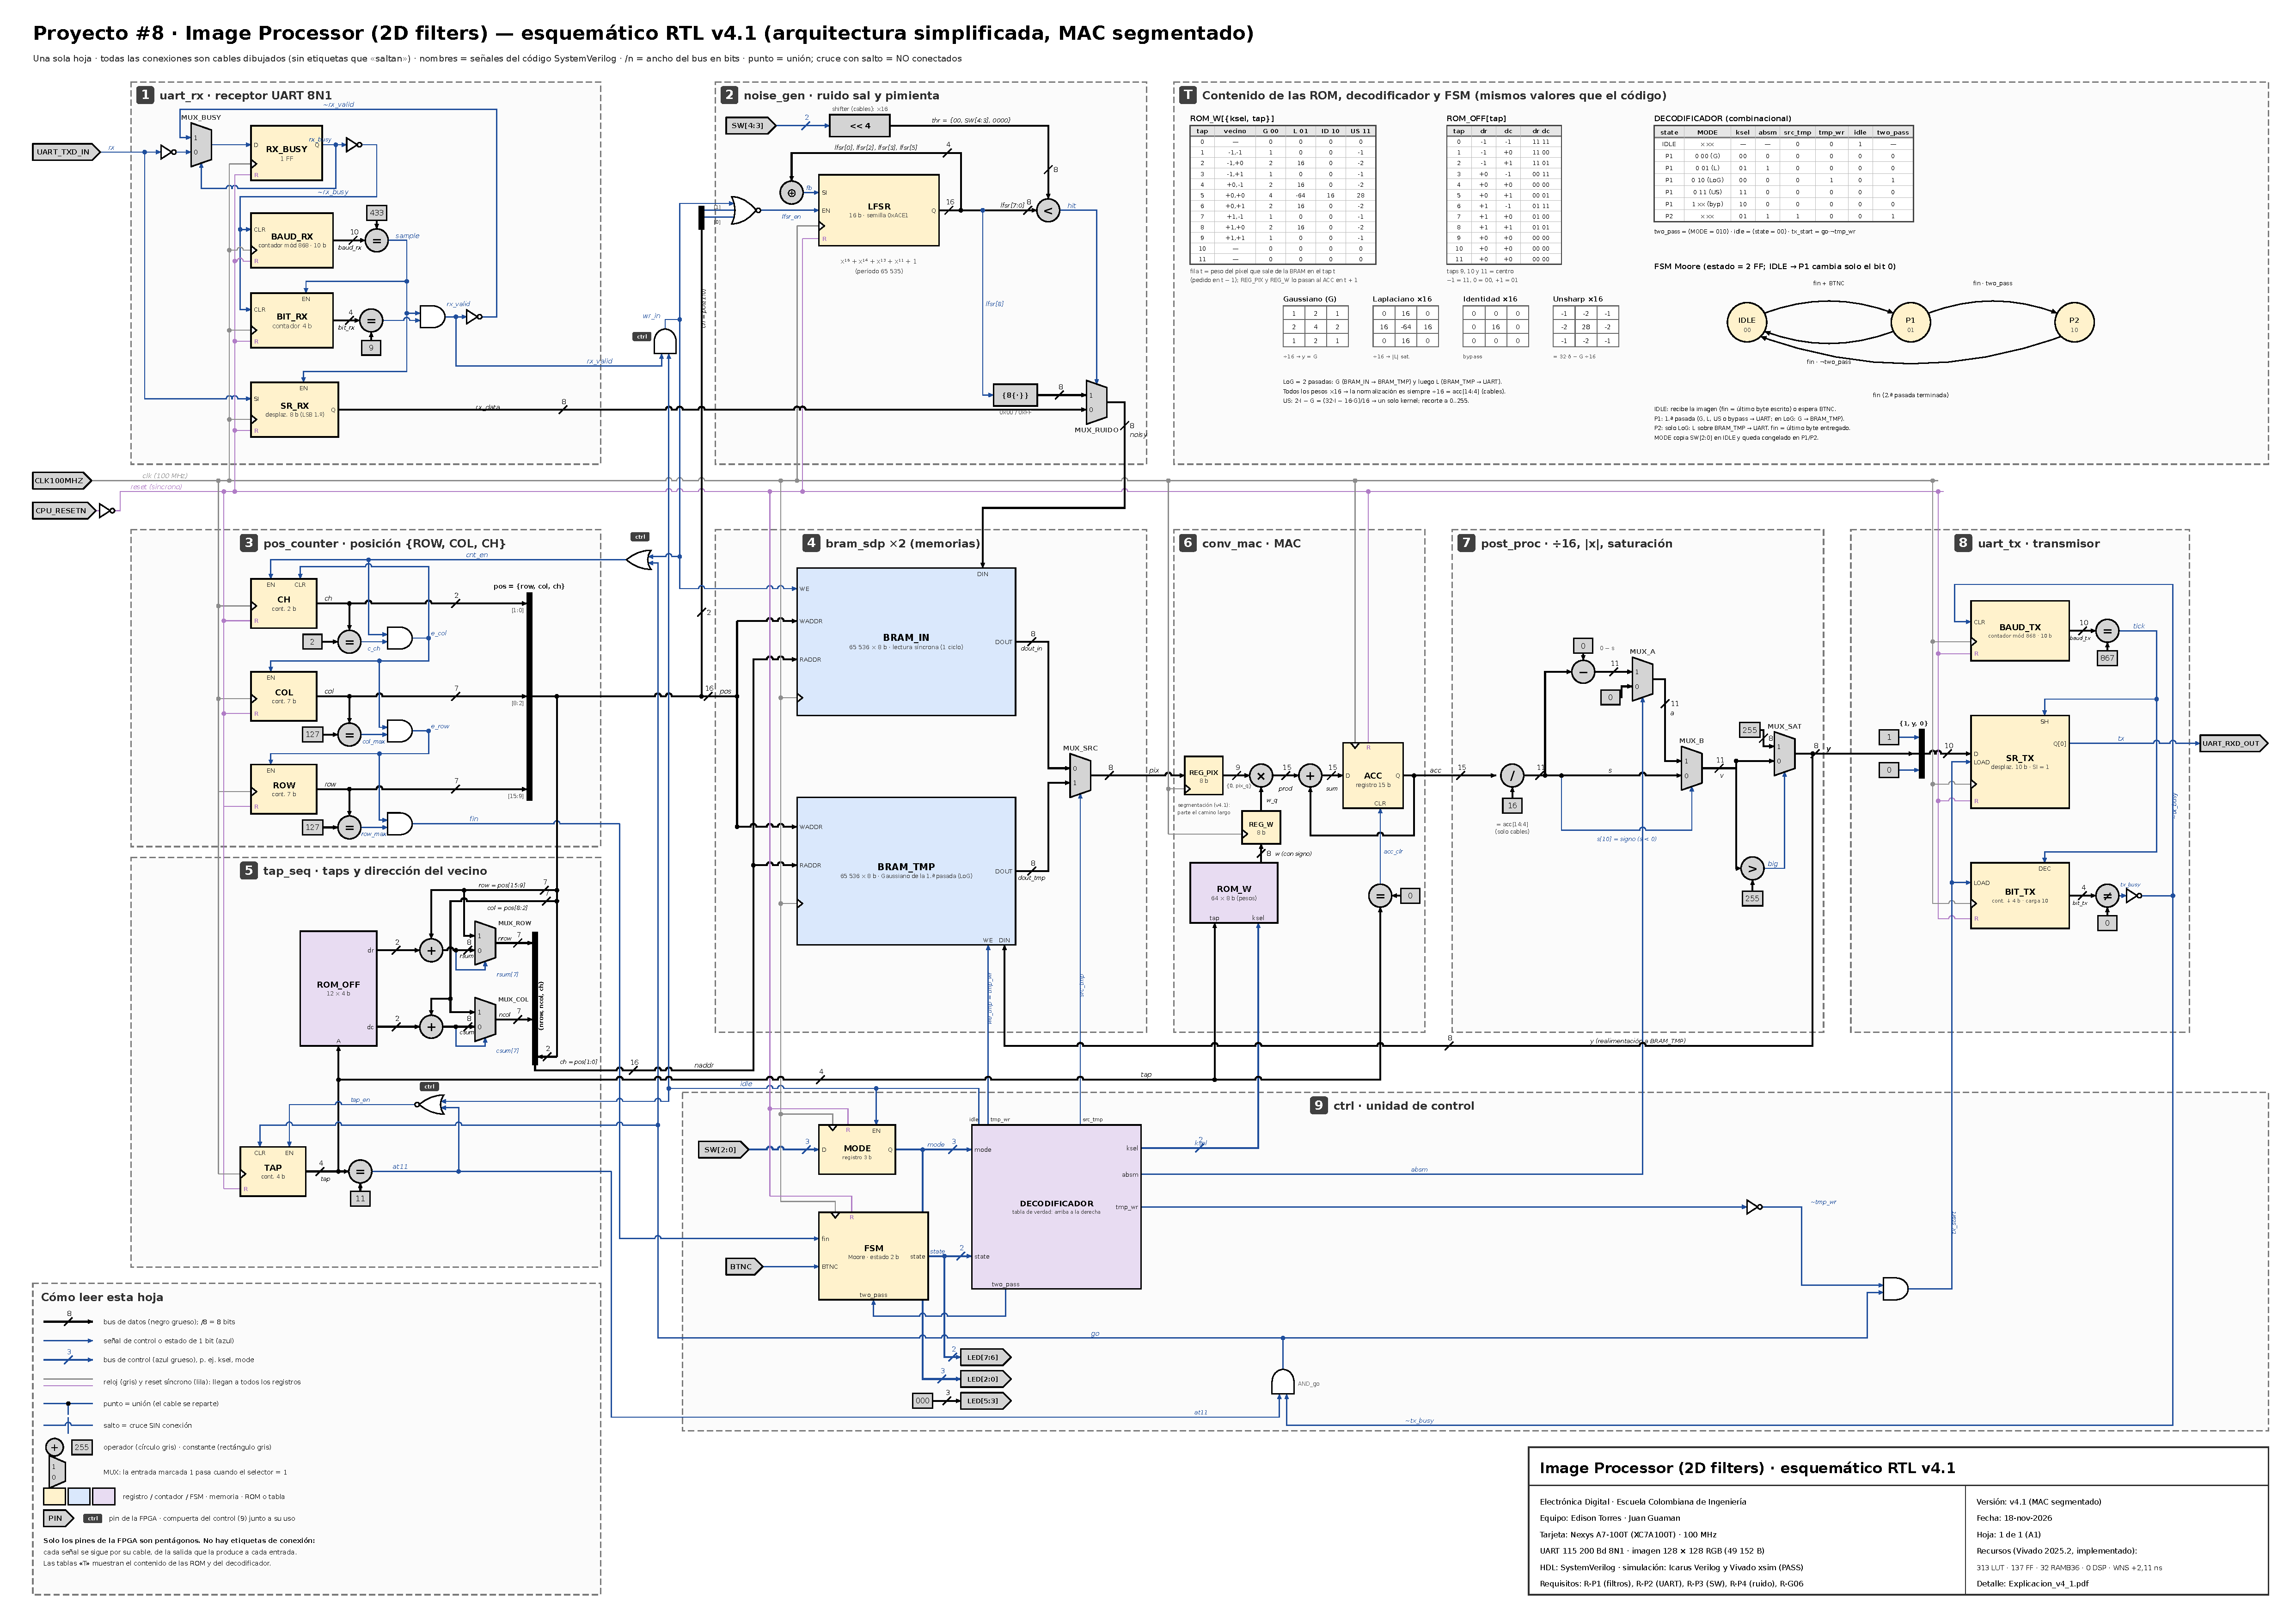
\includegraphics[width=\linewidth,height=0.92\textwidth,keepaspectratio]{../esquematico/esquematico_v4_1.pdf}
\caption{Esquemático RTL v4.1 completo (reducido; ver \texttt{esquematico\_v4\_1.pdf} en A1).}
\label{fig:esq}
\end{figure}
\end{landscape}

\subsection{Cómo leer el esquemático}
\begin{itemize}
\item \textbf{Negro grueso:} bus de datos, con su ancho en bits (\,/8 = 8 bits). \textbf{Azul fino:} señal de control o de estado de 1 bit. \textbf{Azul grueso:} bus de control (\sig{ksel}, \sig{mode}, \sig{state}).
\item \textbf{Gris y lila:} reloj y reset síncrono. Llegan a todos los registros por ``peines'': una línea vertical por bloque y un ramal a cada registro (triángulo = entrada de reloj, R = reset).
\item \textbf{Punto:} unión (la señal se reparte). \textbf{Salto (pequeño arco):} los cables se cruzan \emph{sin} conectarse.
\item Notación de la guía del profesor (\texttt{5\_Implementacion\_Operaciones\_Puntuales}): operadores en círculos grises, constantes en rectángulos grises, MUX trapezoidales con la entrada 1 y la entrada 0 marcadas.
\item \textbf{Amarillo:} registros, contadores y la FSM. \textbf{Azul claro:} memorias. \textbf{Lila:} ROM y decodificador (tablas).
\item Las compuertas con la marca \textbf{ctrl} pertenecen a la unidad de control, pero están dibujadas junto al bloque que usa su salida para que el cable sea corto.
\end{itemize}

% =====================================================================
\section{Tabla de conexiones (de dónde sale y a dónde llega cada señal)}
Esta tabla es el ``índice'' del esquemático: permite comprobar que cada señal tiene un único origen y todos sus destinos dibujados.

{\small
\begin{longtable}{>{\ttfamily}l c >{\raggedright\arraybackslash}p{3.6cm} >{\raggedright\arraybackslash}p{6.45cm}}
\toprule
\normalfont\textbf{Señal} & \textbf{Bits} & \textbf{Sale de} & \textbf{Llega a} \\
\midrule
\endhead
rx (UART\_TXD\_IN) & 1 & pin & NOT $\to$ MUX\_BUSY (entrada 0); SI de SR\_RX \\
rx\_busy & 1 & RX\_BUSY & selector de MUX\_BUSY; NOT $\to$ \texttt{\textasciitilde rx\_busy} \\
\textasciitilde rx\_busy & 1 & NOT & CLR de BAUD\_RX y de BIT\_RX \\
baud\_rx & 10 & BAUD\_RX & comparador $= 433$ \\
sample & 1 & comparador $= 433$ & EN de BIT\_RX; EN de SR\_RX; AND de \texttt{rx\_valid} \\
bit\_rx & 4 & BIT\_RX & comparador $= 9$ \\
rx\_valid & 1 & AND & NOT $\to$ MUX\_BUSY (entrada 1); AND\_wr \\
rx\_data & 8 & SR\_RX & MUX\_RUIDO (entrada 0) \\
idle & 1 & decodificador & AND\_wr; NOR de \texttt{tap\_en}; EN de MODE \\
wr\_in & 1 & AND\_wr (ctrl) & WE de BRAM\_IN; OR\_cnt; NOR de \texttt{lfsr\_en} \\
lfsr & 16 & LFSR & [7:0] $\to$ comparador $<$; [8] $\to$ \{8\{·\}\}; [0], [2], [3], [5] $\to$ $\oplus$ \\
fb & 1 & $\oplus$ (XOR de 4) & SI del LFSR \\
lfsr\_en & 1 & NOR de 3 & EN del LFSR \\
thr & 8 & shifter $\ll4$ (\texttt{SW[4:3]}) & comparador $<$ \\
hit & 1 & comparador $<$ & selector de MUX\_RUIDO \\
noisy & 8 & MUX\_RUIDO & DIN de BRAM\_IN \\
cnt\_en & 1 & OR\_cnt (ctrl) & EN de CH; AND de \texttt{e\_col} \\
ch, col, row & 2, 7, 7 & contadores CH, COL, ROW & comparadores $= 2$, $= 127$, $= 127$; barra \texttt{pos} \\
c\_ch, col\_max, row\_max & 1 & comparadores & AND de \texttt{e\_col}, \texttt{e\_row}, \texttt{fin} \\
e\_col & 1 & AND & CLR de CH; EN de COL; AND de \texttt{e\_row} \\
e\_row & 1 & AND & EN de ROW; AND de \texttt{fin} \\
fin & 1 & AND & entrada \texttt{fin} de la FSM \\
pos & 16 & barra \{row, col, ch\} & WADDR de BRAM\_IN y BRAM\_TMP; bloque 5 (row, col, ch); NOR del bloque 2 (\texttt{pos[1:0]}) \\
tap & 4 & TAP & comparador $= 11$; ROM\_OFF; ROM\_W; comparador $= 0$ \\
at11 & 1 & comparador $= 11$ & NOR de \texttt{tap\_en}; AND\_go \\
tap\_en & 1 & NOR (ctrl) & EN de TAP \\
go & 1 & AND\_go & CLR de TAP; OR\_cnt; AND de \texttt{tx\_start} \\
dr, dc & 2, 2 & ROM\_OFF & sumadores de fila y columna \\
rsum, csum & 8, 8 & sumadores & MUX\_ROW, MUX\_COL (entrada 0); bit 7 $\to$ selector \\
nrow, ncol & 7, 7 & MUX\_ROW, MUX\_COL & barra \texttt{naddr} \\
naddr & 16 & barra \{nrow, ncol, ch\} & RADDR de BRAM\_IN y BRAM\_TMP \\
dout\_in, dout\_tmp & 8, 8 & BRAM\_IN, BRAM\_TMP & MUX\_SRC (entradas 0 y 1) \\
src\_tmp & 1 & decodificador & selector de MUX\_SRC \\
pix & 8 & MUX\_SRC & D de REG\_PIX \\
pix\_q & 8 & REG\_PIX & multiplicador (como \{0, pix\_q\}, 9\,b) \\
ksel & 2 & decodificador & dirección alta de ROM\_W \\
w & 8 & ROM\_W & D de REG\_W \\
w\_q & 8 & REG\_W & multiplicador \\
prod, sum & 15, 15 & multiplicador, sumador & sumador; D del ACC \\
acc\_clr & 1 & comparador $= 0$ & CLR del ACC \\
acc & 15 & ACC & sumador (realimentación); divisor $\div16$ \\
s & 11 & $\div16$ (cables) & negador; MUX\_B (entrada 0); \texttt{s[10]} $\to$ selector de MUX\_B \\
$-$s, a, v & 11 & negador, MUX\_A, MUX\_B & MUX\_A (1); MUX\_B (1); MUX\_SAT (0) y comparador $>$ \\
absm & 1 & decodificador & selector de MUX\_A \\
big & 1 & comparador $> 255$ & selector de MUX\_SAT \\
y & 8 & MUX\_SAT & barra \{1, y, 0\} $\to$ D de SR\_TX; DIN de BRAM\_TMP \\
tmp\_wr & 1 & decodificador & WE de BRAM\_TMP; NOT $\to$ AND de \texttt{tx\_start} \\
tx\_start & 1 & AND (ctrl) & LOAD de SR\_TX y de BIT\_TX \\
tick & 1 & comparador $= 867$ & SH de SR\_TX; DEC de BIT\_TX \\
bit\_tx, baud\_tx & 4, 10 & BIT\_TX, BAUD\_TX & comparadores $\neq 0$ y $= 867$ \\
tx\_busy & 1 & comparador $\neq 0$ & NOT $\to$ \texttt{\textasciitilde tx\_busy} \\
\textasciitilde tx\_busy & 1 & NOT & CLR de BAUD\_TX; AND\_go \\
tx (UART\_RXD\_OUT) & 1 & \texttt{SR\_TX[0]} & pin \\
mode & 3 & MODE & decodificador; \texttt{LED[2:0]} \\
state & 2 & FSM & decodificador; \texttt{LED[7:6]} \\
two\_pass & 1 & decodificador & FSM \\
\bottomrule
\end{longtable}
}

% =====================================================================
\section{Bloque por bloque}

\subsection{Bloque 1 — \texorpdfstring{\texttt{uart\_rx}}{uart\_rx}: receptor UART 8N1}
\begin{center}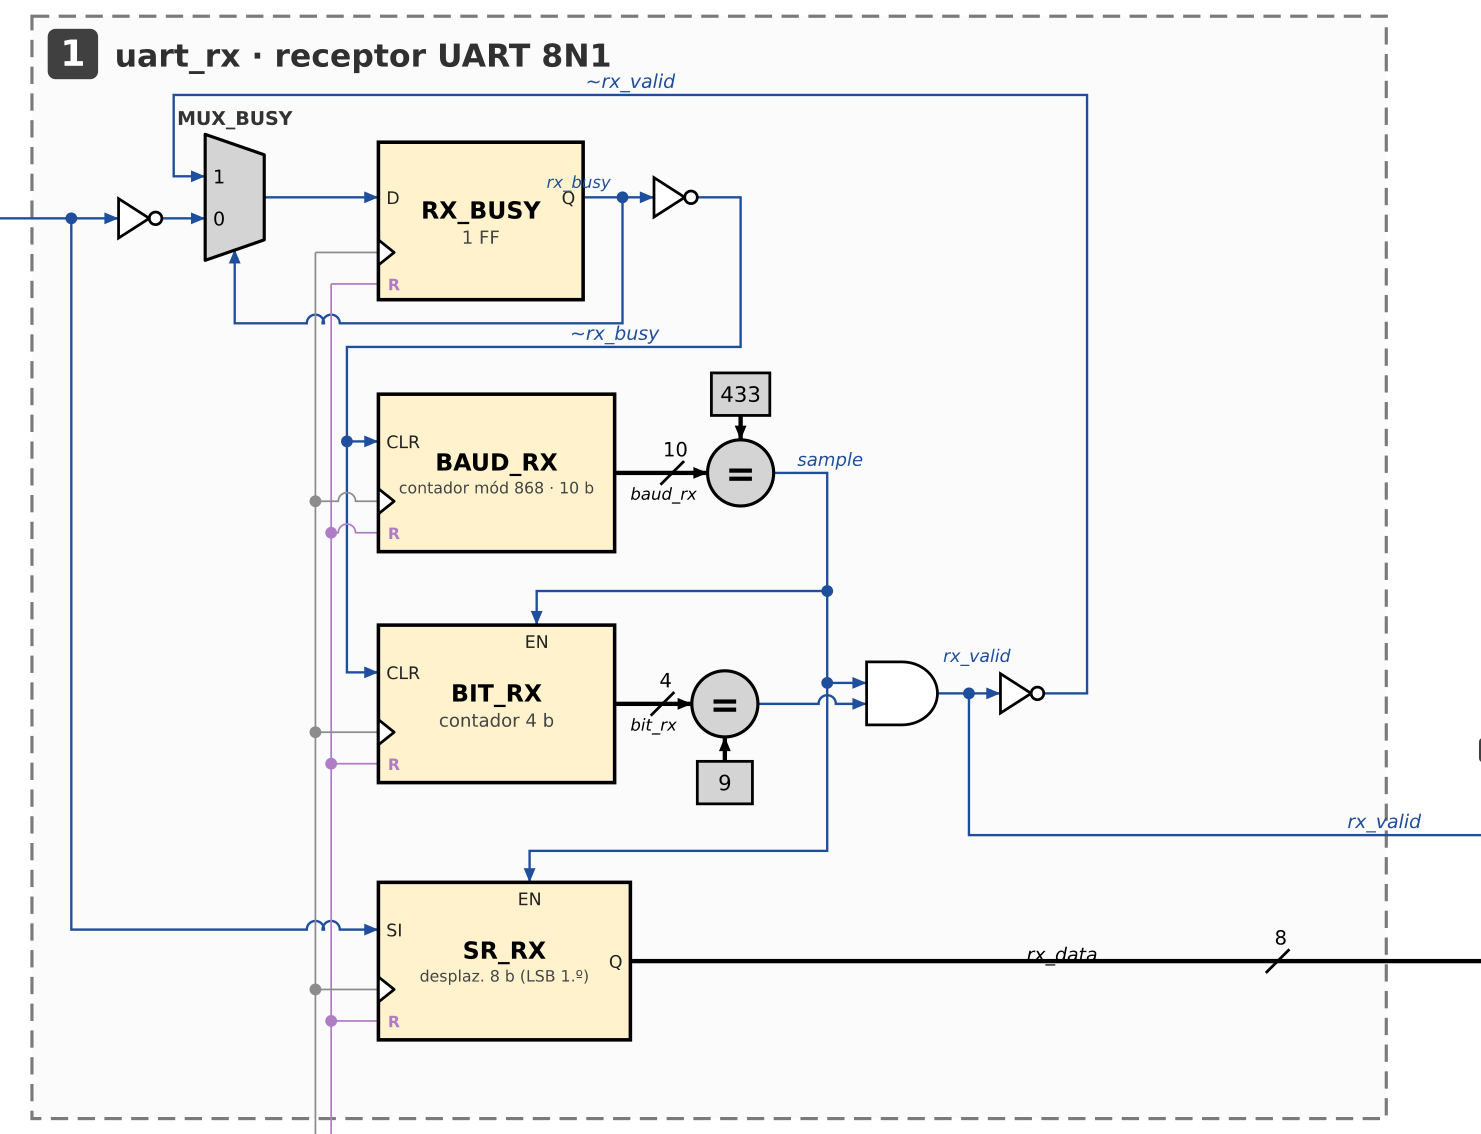
\includegraphics[width=0.92\linewidth]{img/blk1.png}\end{center}

\textbf{Qué hace.} Convierte la línea serie \bus{UART\_TXD\_IN} en bytes. Una trama 8N1 es: bit de inicio (0), 8 bits de datos con el LSB primero y bit de parada (1); cada bit dura 868 ciclos.

\textbf{Hardware.}
\begin{itemize}
\item \textbf{RX\_BUSY} (1 FF) indica que se está recibiendo un byte. Su entrada es MUX\_BUSY: si \sig{rx\_busy} = 0, el siguiente valor es $\overline{rx}$ (la línea bajó $\Rightarrow$ empieza un byte); si \sig{rx\_busy} = 1, es $\overline{rx\_valid}$ (al muestrear el bit de parada se termina el byte).
\item \textbf{BAUD\_RX}: contador módulo 868 (10\,b; $2^{10} = 1024 > 868$). Se borra mientras \sig{rx\_busy} = 0, así que empieza en 0 justo en el flanco de inicio.
\item Comparador \textbf{$=433$} $\Rightarrow$ \sig{sample}: marca la \emph{mitad} de cada bit (433 ciclos después de su comienzo), el punto más alejado de los flancos.
\item \textbf{BIT\_RX}: cuenta las muestras (4\,b): 0 = inicio, 1–8 = datos, 9 = parada.
\item \textbf{SR\_RX}: registro de desplazamiento de 8\,b; en cada muestra entra \bus{rx} por el MSB y todo se corre a la derecha. Tras las muestras 0…8, el bit de inicio ya salió por la derecha y quedan \bus{d7…d0} en su lugar.
\item AND: \sig{rx\_valid} $=$ \sig{sample} $\cdot$ (\bus{bit\_rx} $= 9$). En ese ciclo \bus{rx\_data} ya tiene el byte completo (el desplazamiento de la muestra 9 ocurre en el flanco siguiente, cuando el byte ya se guardó).
\end{itemize}

\textbf{Decisiones y alternativas.}
\begin{itemize}
\item \emph{FSM de 4 estados (v3) frente a RX\_BUSY + contadores (v4).} Ambas son correctas. La v4 tiene un FF menos de estado y no requiere diagrama de estados: el ``estado'' es el número de muestra (\bus{bit\_rx}).
\item \emph{Sin verificación del bit de inicio a mitad de bit.} Una UART más robusta comprobaría que la línea sigue en 0 en la muestra 0 (rechazo de falsos inicios). El cable USB-UART es limpio y la línea en reposo es 1; se prefirió el diseño mínimo. Si ven bytes falsos al conectar el cable, esta es la primera mejora a considerar.
\item \emph{Sin sincronizador (D15).} Mientras \sig{rx\_busy} = 0, la entrada asíncrona solo llega a un FF (RX\_BUSY); durante el byte solo se lee a mitad de bit, cuando la línea está estable.
\end{itemize}

\textbf{Verificación (\texttt{tb\_uart\_rx}, con 868 ciclos por bit reales):} los 256 valores seguidos sin pausa, 64 bytes con pausas aleatorias, error de reloj de $+3$\,\% y $-3$\,\%, latencia de \sig{rx\_valid} = 8\,246 ciclos = 9,5 bits (justo en la mitad del bit de parada), reposo largo sin bytes falsos y reset en medio de un byte (aparece 1 byte basura, como en cualquier UART; después 8 de 8 correctos). Resultado: PASS.

\subsection{Bloque 2 — \texorpdfstring{\texttt{noise\_gen}}{noise\_gen}: ruido sal y pimienta (R-P4)}
\begin{center}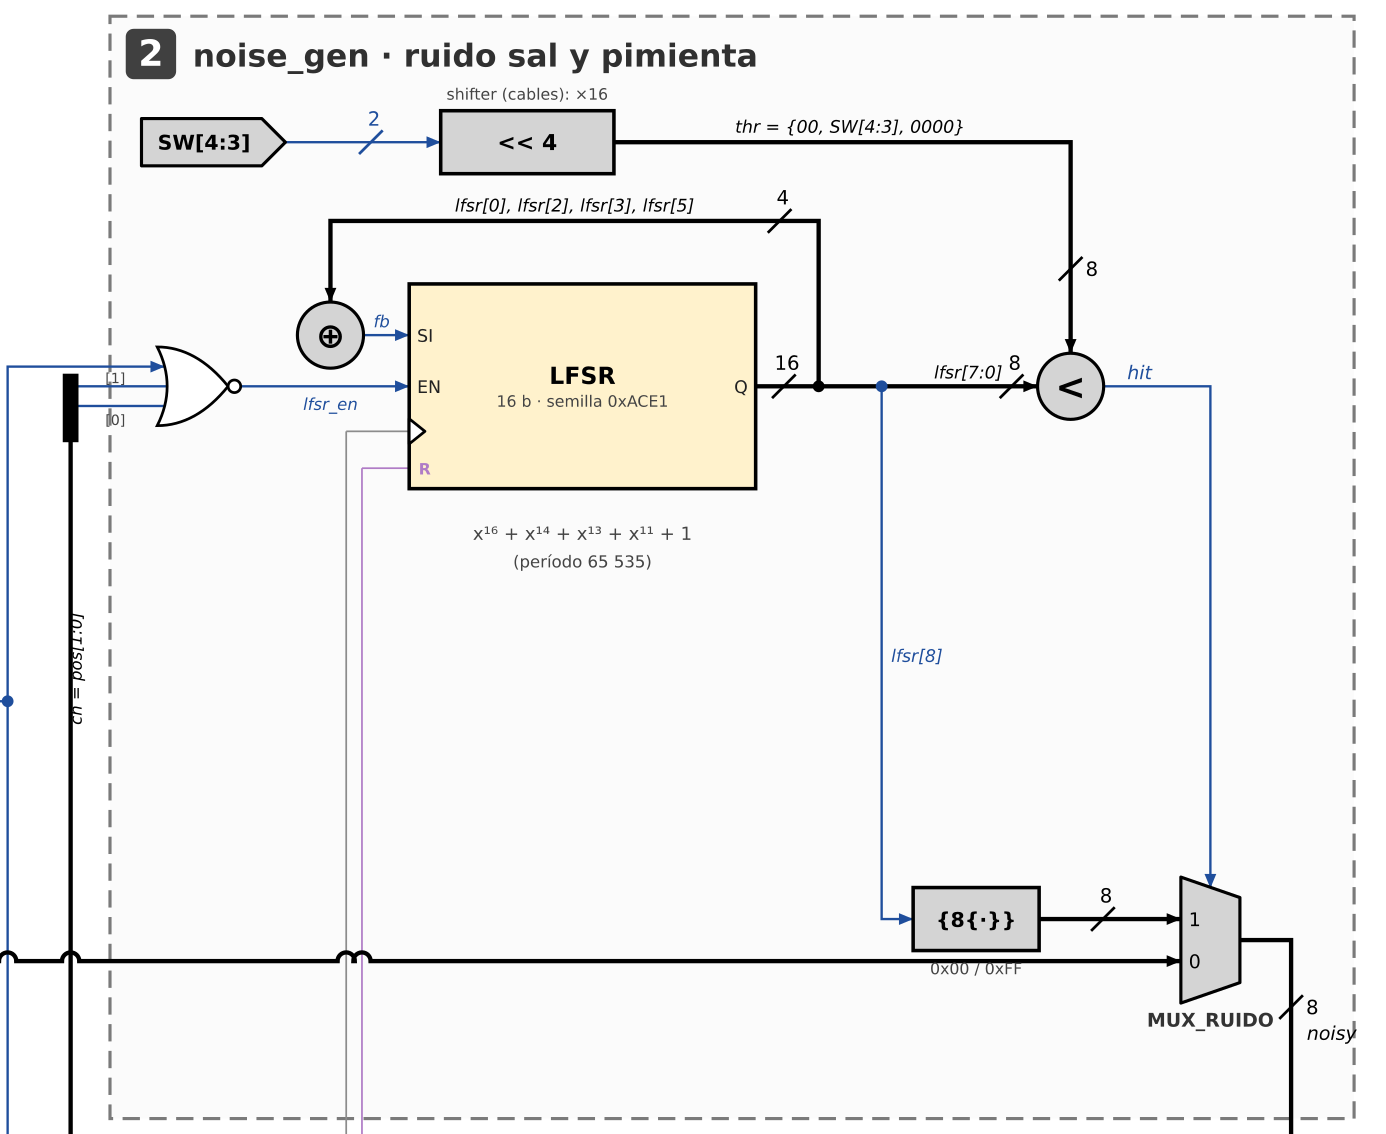
\includegraphics[width=0.85\linewidth]{img/blk2.png}\end{center}

\textbf{Qué hace.} Con probabilidad \bus{thr}/256 reemplaza el píxel recibido por blanco (0xFF) o negro (0x00). El ruido se aplica al recibir, así que BRAM\_IN guarda la imagen con ruido y todos los filtros (y el bypass) trabajan sobre ella.

\textbf{Hardware.}
\begin{itemize}
\item \textbf{LFSR} de 16\,b (registro de desplazamiento a la derecha) con realimentación \sig{fb} $=$ \bus{lfsr[0]} $\oplus$ \bus{lfsr[2]} $\oplus$ \bus{lfsr[3]} $\oplus$ \bus{lfsr[5]}, que corresponde al polinomio $x^{16}+x^{14}+x^{13}+x^{11}+1$. Recorre los $2^{16}-1 = 65\,535$ estados distintos de cero (verificado en simulación). Semilla \texttt{0xACE1}.
\item Shifter \textbf{$\ll 4$}: \bus{thr} $=$ \{00, \bus{SW[4:3]}, 0000\} $=$ \bus{SW[4:3]} $\times 16 \in \{0, 16, 32, 48\}$. Son solo cables.
\item Comparador \textbf{$<$}: \sig{hit} $=$ (\bus{lfsr[7:0]} $<$ \bus{thr}). Como los 8 bits bajos del LFSR son prácticamente uniformes, $P(\text{hit}) = \text{thr}/256$.
\item \textbf{\{8\{·\}\}}: repite \bus{lfsr[8]} 8 veces $\Rightarrow$ 0x00 (pimienta) o 0xFF (sal). Son cables.
\item \textbf{MUX\_RUIDO} (8\,b): \bus{noisy} $=$ \sig{hit} ? \{8\{\bus{lfsr[8]}\}\} : \bus{rx\_data}.
\item \textbf{NOR de 3 entradas}: \sig{lfsr\_en} $= \overline{ch[1] + ch[0] + wr\_in}$.
\end{itemize}

\textbf{¿Por qué el LFSR se congela durante el píxel?} Los tres bytes de un píxel (R, G, B) deben recibir la \emph{misma} decisión; si no, el ruido saldría de colores. El LFSR corre libre mientras se espera el byte R (\bus{ch} = 0 y sin escritura) y se detiene desde la escritura de R hasta la de B: los tres bytes ven el mismo estado.

\textbf{¿Por qué libre y no ``un paso por píxel''?} Con un solo desplazamiento por píxel, dos decisiones seguidas comparten 7 de los 8 bits que se comparan: si un píxel tiene ruido, el siguiente lo tiene con probabilidad 1/2 y el ruido aparece en ``rayitas'' horizontales. Corriendo libre, entre dos píxeles pasan miles de desplazamientos y las decisiones son independientes. \emph{Consecuencia:} el patrón de ruido depende de cuándo empieza a enviar el PC, así que cambia en cada envío.

\textbf{Verificación (\texttt{tb\_noise\_gen}):} período exacto de 65\,535; en un período completo hay exactamente 0, 4\,095, 8\,191 y 12\,287 aciertos para los cuatro niveles (con thr $> 0$ hay $256\cdot\text{thr}$ estados cuyo byte bajo es menor que thr, menos el estado 0, que el LFSR nunca toma: $256\cdot\text{thr} - 1$); 200\,000 ciclos con entradas aleatorias comparados contra un modelo independiente; 3\,000 píxeles: todos los que reciben ruido quedan completamente blancos o negros. PASS.

\subsection{Bloque 3 — \texorpdfstring{\texttt{pos\_counter}}{pos\_counter}: contador de posición \{ROW, COL, CH\}}
\begin{center}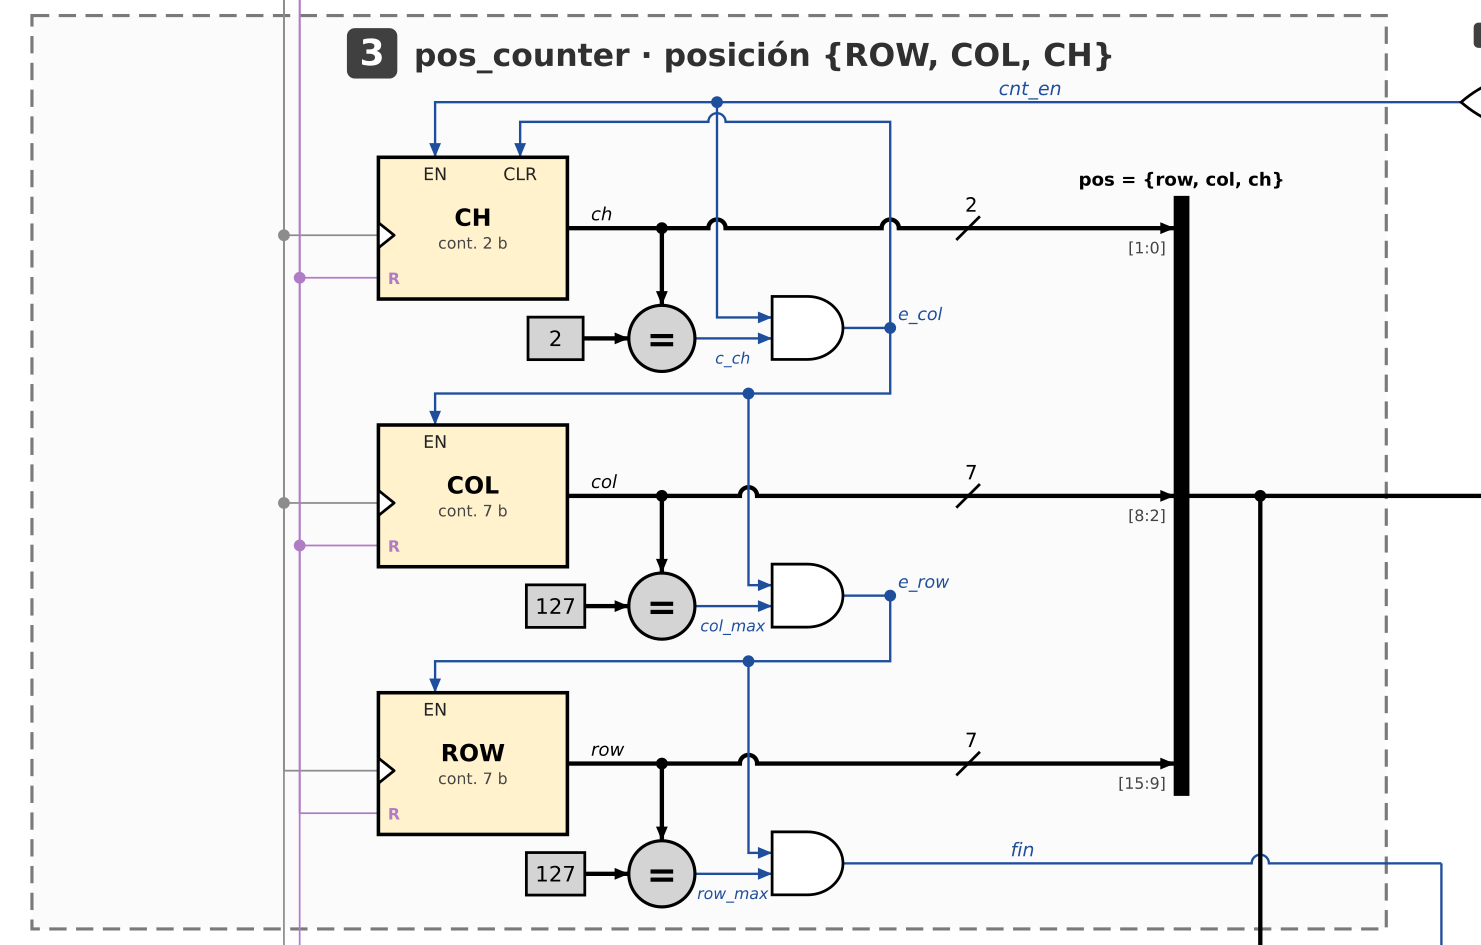
\includegraphics[width=0.78\linewidth]{img/blk3.png}\end{center}

\textbf{Qué hace.} Lleva la cuenta de \emph{qué byte} se está escribiendo (al recibir) o calculando (al procesar), en el orden de la UART: canal R, G, B; luego la siguiente columna; luego la siguiente fila. La concatenación \bus{pos} $=$ \{row, col, ch\} (16\,b) es la dirección de escritura de las dos memorias.

\textbf{Hardware.} Tres contadores en cascada:
\begin{itemize}
\item \textbf{CH} (2\,b) avanza con \sig{cnt\_en} y se borra con \sig{e\_col}: cuenta 0, 1, 2, 0, …
\item \textbf{COL} (7\,b) avanza con \sig{e\_col} $=$ \sig{cnt\_en} $\cdot$ (\bus{ch} $= 2$).
\item \textbf{ROW} (7\,b) avanza con \sig{e\_row} $=$ \sig{e\_col} $\cdot$ (\bus{col} $= 127$).
\item \sig{fin} $=$ \sig{e\_row} $\cdot$ (\bus{row} $= 127$): la cuenta avanza \emph{desde} el último byte de la imagen.
\end{itemize}
COL y ROW vuelven solos a 0 porque $127 + 1 = 0$ en 7 bits; no necesitan comparador para la vuelta.

\textbf{Un solo contador para dos trabajos.} \sig{cnt\_en} $=$ \sig{wr\_in} $+$ \sig{go} (compuerta OR\_cnt, marcada ctrl). En IDLE solo puede haber \sig{wr\_in} (se recibe); en P1/P2 solo \sig{go} (se calcula). Por eso \sig{fin} significa ``imagen recibida'' en IDLE y ``pasada terminada'' en P1/P2, y la FSM usa una sola señal para ambos casos.

\textbf{Verificación (\texttt{tb\_pos\_counter}):} dos instancias (128\,×\,128 y 8\,×\,8) con enable aleatorio y dos barridos completos: orden R, G, B $\to$ columna $\to$ fila, \sig{fin} solo al avanzar desde (2, 127, 127), vuelta a (0, 0, 0) y enable en 0 congela la cuenta. PASS.

\subsection{Bloque 4 — \texorpdfstring{\texttt{bram\_sdp}}{bram\_sdp} ×2: memorias de imagen}
\begin{center}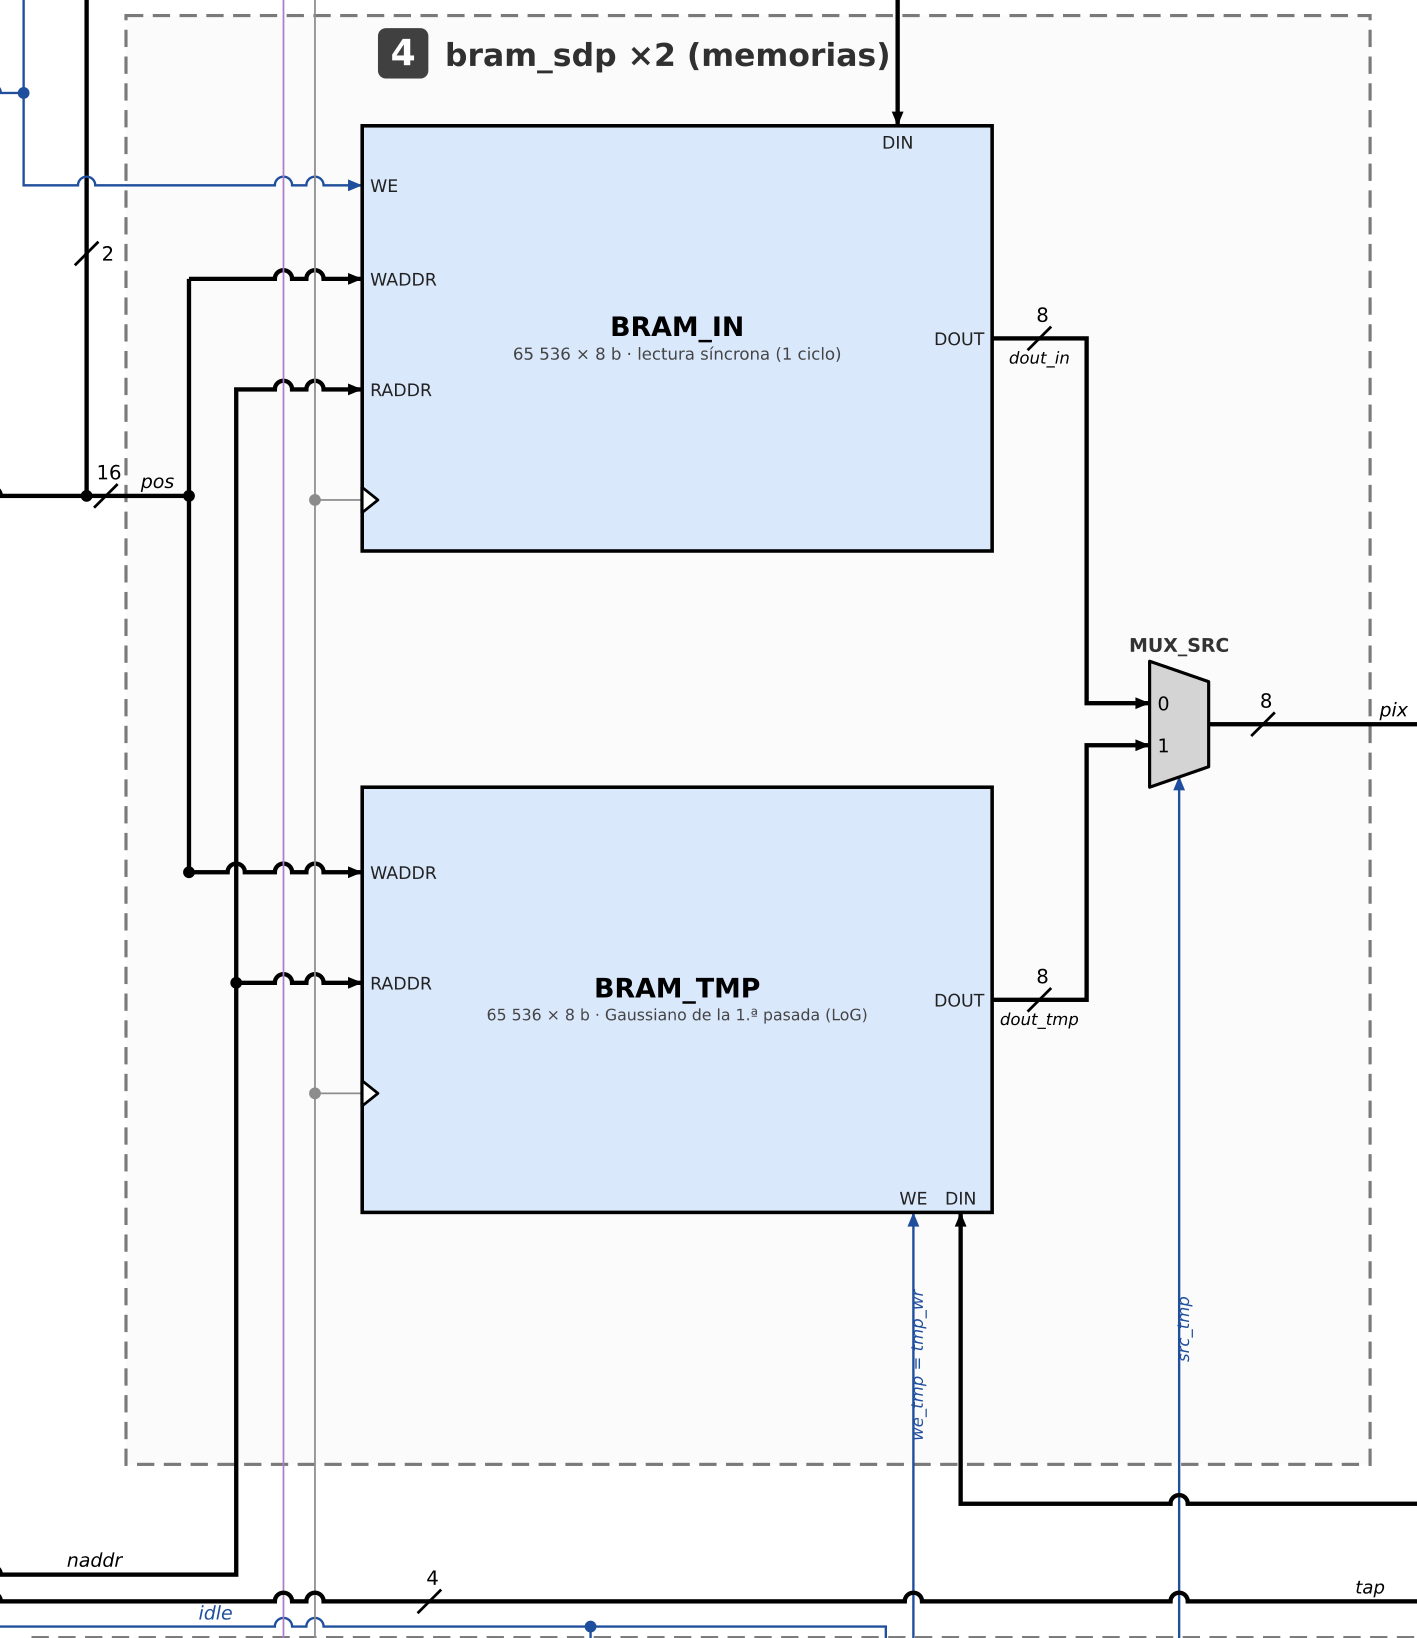
\includegraphics[width=0.62\linewidth]{img/blk4.png}\end{center}

\textbf{Qué hace.} BRAM\_IN guarda la imagen recibida (con ruido). BRAM\_TMP guarda el Gaussiano de la primera pasada del LoG. Son memorias de doble puerto simple: un puerto de escritura (WE, WADDR, DIN) y uno de lectura (RADDR, DOUT) que funcionan a la vez.

\textbf{Detalles importantes.}
\begin{itemize}
\item \textbf{Lectura síncrona:} el dato aparece un ciclo después de presentar la dirección. Así Vivado infiere Block RAM. Es la razón de que el MAC trabaje con retraso respecto al tap que pide la dirección (bloque 6).
\item \textbf{Tamaño:} 65\,536 × 8\,b cada una (dirección de 16\,b). Las direcciones con canal = 3 nunca se usan. Vivado usa 16 RAMB36 por memoria (32 en total), el 23,7\,\% de los 135 bloques que su reporte de utilización da para la XC7A100T.
\item \textbf{Escrituras:} BRAM\_IN con \sig{wr\_in}; BRAM\_TMP con \sig{tmp\_wr}, es decir, en \emph{todos} los ciclos de la pasada P1 del LoG. Mientras se calcula el byte $k$ se escriben valores intermedios en la dirección $k$, pero la última escritura en esa dirección ocurre en el ciclo de \sig{go}, con el resultado correcto. Así no hace falta una AND con \sig{go}.
\item \textbf{MUX\_SRC} elige de qué memoria lee el MAC: BRAM\_IN (0) o BRAM\_TMP (1, solo en P2).
\item Durante la pasada que escribe BRAM\_TMP (P1 del LoG) el MAC lee de BRAM\_IN, así que lo que salga del puerto de lectura de BRAM\_TMP en esos ciclos nunca se usa: una lectura y una escritura simultáneas en la misma dirección no afectan el resultado.
\end{itemize}

\textbf{Verificación (\texttt{tb\_bram\_sdp}):} 300\,000 ciclos de tráfico aleatorio, latencia de 1 ciclo, extremos 0 y 65\,535, escritura de toda la memoria y lectura completa. PASS.

\subsection{Bloque 5 — \texorpdfstring{\texttt{tap\_seq}}{tap\_seq}: taps y dirección del vecino}
\begin{center}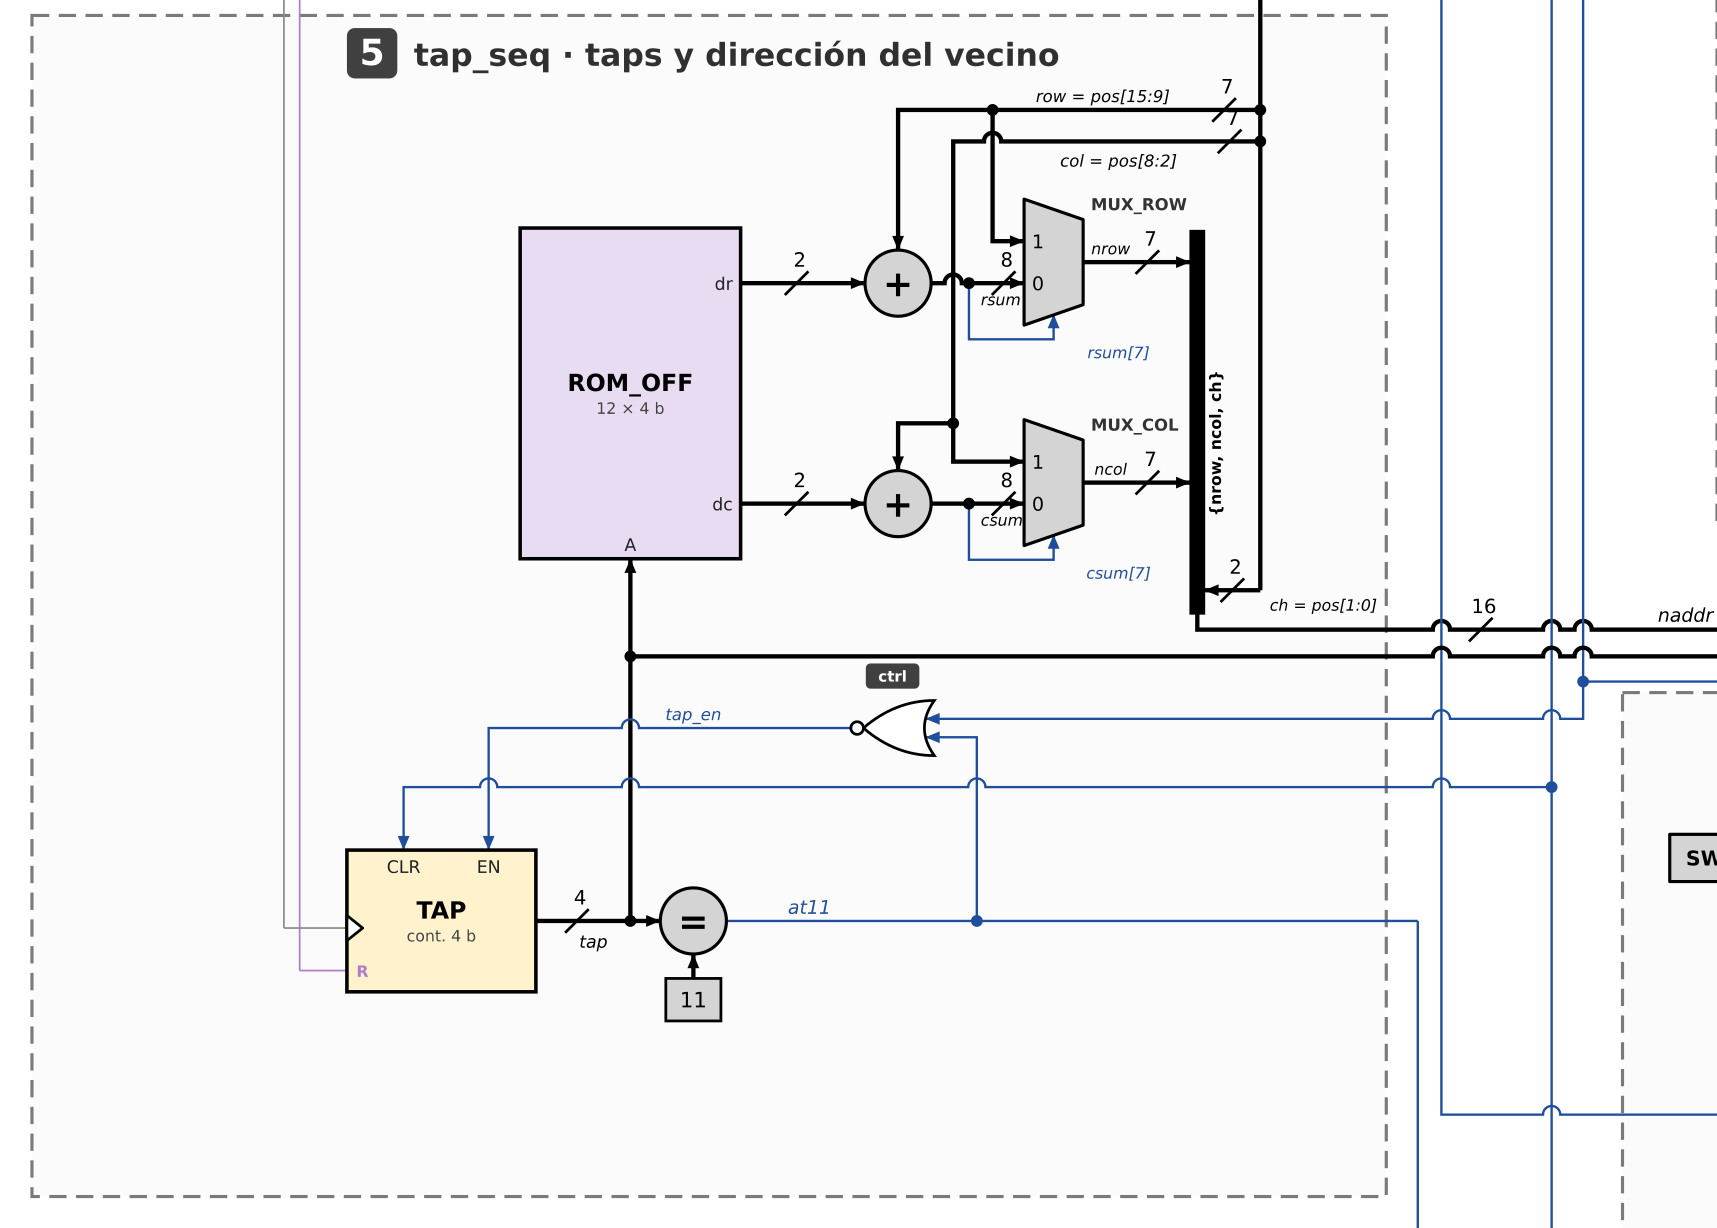
\includegraphics[width=0.80\linewidth]{img/blk5.png}\end{center}

\textbf{Qué hace.} Genera, ciclo a ciclo, la dirección \bus{naddr} de cada uno de los 9 vecinos del byte actual, replicando el borde de la imagen (D1).

\textbf{Hardware.}
\begin{itemize}
\item \textbf{TAP} (4\,b): CLR $=$ \sig{go}; EN $=$ \sig{tap\_en} $= \overline{at11 + idle}$ (NOR marcada ctrl). Cuenta 0…11, se queda en 11 hasta que llega \sig{go} y no cuenta en IDLE.
\item Comparador \textbf{$=11$} $\Rightarrow$ \sig{at11}: el resultado del byte está listo (en v4 era $=10$; ver sección~\ref{sec:tiempos}).
\item \textbf{ROM\_OFF} (12 × 4\,b): convierte el tap en el desplazamiento del vecino, $(dr, dc) \in \{-1, 0, +1\}^2$ en complemento a 2 de 2\,b ($-1 = 11$, $0 = 00$, $+1 = 01$). Taps 0–8 en orden de barrido; 9, 10 y 11 apuntan al centro.
\item Separación de \bus{pos}: \bus{row} $=$ \bus{pos[15:9]}, \bus{col} $=$ \bus{pos[8:2]}, \bus{ch} $=$ \bus{pos[1:0]}.
\item \textbf{Sumadores de 8\,b} y \textbf{MUX\_ROW / MUX\_COL}: \bus{rsum} $= \{0, \text{row}\} + \text{ext}(dr)$; si \bus{rsum[7]} $= 1$ el vecino está fuera de la imagen y el MUX deja la fila actual (``si se sale, no se mueve'').
\end{itemize}

\textbf{¿Por qué basta el bit 7?} La fila está en $[0, 127]$ y $dr \in \{-1, 0, +1\}$, así que la suma está en $[-1, 128]$. En 8\,bits con complemento a 2:
\[
-1 = 1111\,1111_2, \qquad 0 \ldots 127 = 0\text{xxx}\,\text{xxxx}_2, \qquad 128 = 1000\,0000_2 .
\]
El MSB vale 1 exactamente en los dos casos inválidos. No hacen falta los comparadores ``fila $= 0$'' y ``fila $= 127$'' de la v3.

\textbf{Verificación (\texttt{tb\_tap\_seq}):} \emph{exhaustiva}: las 16\,384 posiciones de 128\,×\,128 (incluidas las 4 esquinas y los 4 bordes), los 3 canales y los 12 taps, comparadas contra $\text{clamp}(\text{fila} + dr)$; espera en 11, borrado con \sig{go} y que en IDLE no cuenta. PASS.

\subsection{Bloque 6 — \texorpdfstring{\texttt{conv\_mac}}{conv\_mac}: convolución 3×3 secuencial}
\begin{center}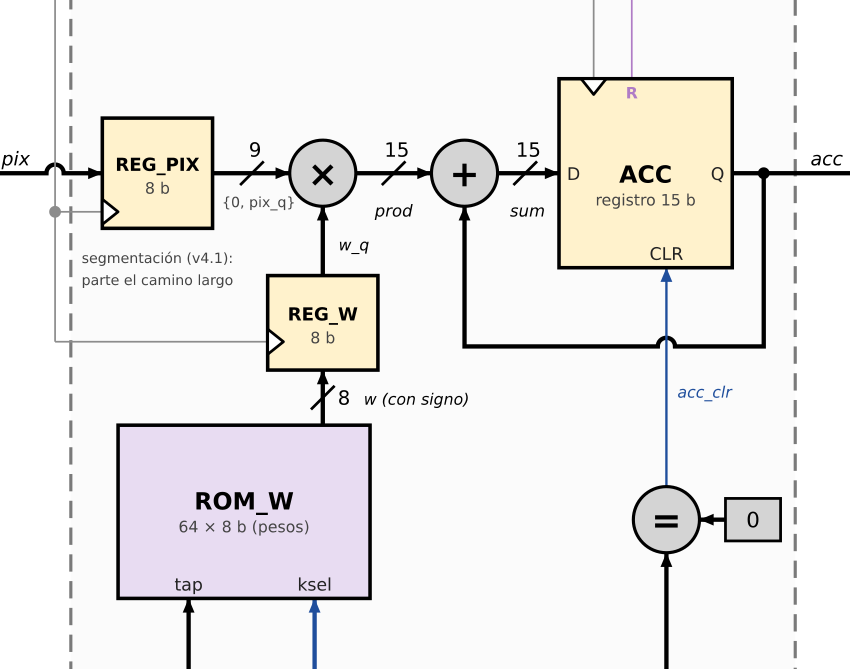
\includegraphics[width=0.78\linewidth]{img/blk6_zoom.png}\end{center}

\textbf{Qué hace.} Calcula $\text{acc} = \sum_{t=0}^{8} K[t]\cdot x_t$ con un solo multiplicador y un solo sumador, un término por ciclo. Desde la v4.1 el píxel y el peso pasan por un registro de segmentación antes de multiplicarse.

\textbf{Hardware.}
\begin{itemize}
\item \textbf{ROM\_W} (dirección \{\sig{ksel}, \bus{tap}\}, 6\,b; dato de 8\,b con signo). La fila $t$ guarda el peso del píxel que \emph{sale de la BRAM} en el tap $t$, es decir, el vecino pedido en el tap $t-1$ (la BRAM tarda un ciclo). Los taps 0, 10 y 11 tienen peso 0.
\item \textbf{REG\_PIX y REG\_W} (8\,b cada uno, v4.1): registran \bus{pix} y \bus{w} en cada flanco. Como se registran juntos, siguen alineados: el producto del vecino pedido en el tap $t$ se acumula al final del tap $t+2$. Parten el camino largo BRAM $\to$ multiplicador $\to$ sumador $\to$ ACC en dos tramos (sección~\ref{sec:tiempos}).
\item \textbf{Multiplicador} con signo: \{0, \bus{pix\_q}\} (9\,b, el 0 delante hace que el píxel se lea como positivo) × \bus{w\_q} (8\,b). Vivado lo implementó con LUT y cadenas de acarreo, sin usar un DSP48.
\item \textbf{Sumador} y \textbf{ACC} (15\,b). ACC se borra cuando \bus{tap} $= 0$ (comparador $=0$ $\Rightarrow$ \sig{acc\_clr}). El borrado en el tap 0 sigue sirviendo con la segmentación: en el tap 1 el peso registrado es ROM\_W[0] $= 0$, así que el primer término que entra es 0. En el tap 11 el peso registrado también es 0 y el ACC se mantiene solo mientras se espera la UART.
\end{itemize}

\textbf{Los cuatro kernels (todos multiplicados por 16).}
\[
G = \begin{bmatrix}1&2&1\\2&4&2\\1&2&1\end{bmatrix},\quad
16L = \begin{bmatrix}0&16&0\\16&-64&16\\0&16&0\end{bmatrix},\quad
16\delta = \begin{bmatrix}0&0&0\\0&16&0\\0&0&0\end{bmatrix},\quad
U = \begin{bmatrix}-1&-2&-1\\-2&28&-2\\-1&-2&-1\end{bmatrix}
\]
El Unsharp con $k = 1$ es $I + (I - G/16) = 2I - G/16 = \tfrac{1}{16}\left(32\,\delta - G\right) * I$: el centro vale $32 - 4 = 28$ y los demás pesos son los del Gaussiano con signo menos. Como todos los kernels están escalados por 16, la normalización es siempre la misma ($\div16$) y se hace con cables en el bloque 7.

\begin{ojo}
\textbf{Tema del curso (para que no los tome por sorpresa).} La presentación 7 (diapositivas 84–86) muestra el multiplicador en arreglo \emph{sin signo}; aquí se usa \emph{con signo}, en complemento a 2. La multiplicación con signo aparece en la presentación 9 (diapositiva 97, instrucciones \texttt{mul} y \texttt{mulh}) y el complemento a 2 en la presentación 7. Si el profesor prefiere quedarse en el multiplicador sin signo, la alternativa es guardar en ROM\_W la magnitud del peso (7\,bits, porque $|w| \le 64$) y un bit de signo, multiplicar sin signo ($8 \times 7$ bits) y convertir el sumador en sumador/restador controlado por ese bit (presentación 7). El resultado es idéntico; cuesta un bit más por fila de la ROM y la lógica de resta.
\end{ojo}

\textbf{Verificación (\texttt{tb\_conv\_mac}):} los 4 kernels con 6 vecindarios extremos (todo 0, todo 255, centro 255, centro 0, dos dameros) y 3\,000 aleatorios cada uno; que el ACC se mantiene en el tap 11 aunque cambie \bus{pix}; rango observado $-16\,320 \ldots 16\,320$. PASS.

\subsection{Bloque 7 — \texorpdfstring{\texttt{post\_proc}}{post\_proc}: \texorpdfstring{$\div16$}{÷16}, valor absoluto y saturación}
\begin{center}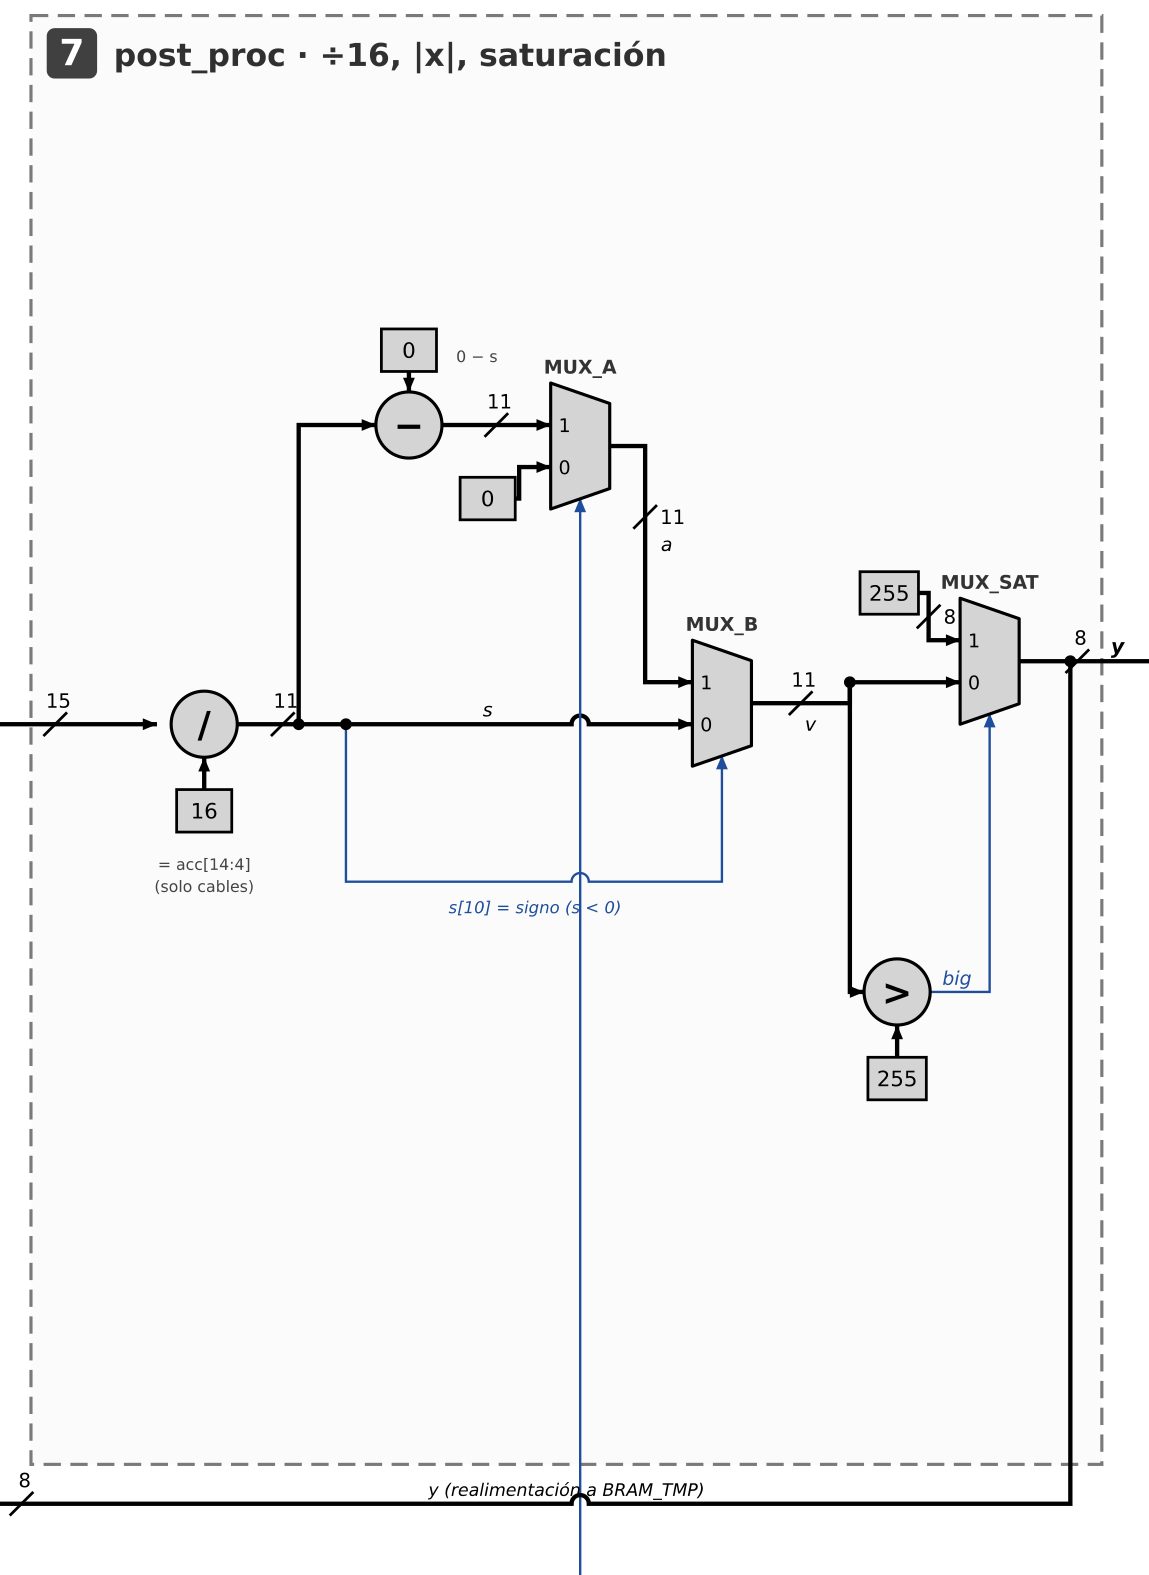
\includegraphics[width=0.60\linewidth]{img/blk7.png}\end{center}

\textbf{Hardware y funcionamiento.}
\begin{itemize}
\item \textbf{$\div 16$}: $s = \lfloor \text{acc}/16 \rfloor = $ \bus{acc[14:4]} (11\,b). Tomar los bits altos de un número en complemento a 2 es un desplazamiento aritmético, $A \ggg 4 = A \div 2^4$ (presentación 7, diapositiva 82), que redondea hacia $-\infty$. Son solo cables.
\item \textbf{Negador} ($0 - s$) y \textbf{MUX\_A}: \bus{a} $=$ \sig{absm} ? $-s$ : 0.
\item \textbf{MUX\_B}: \bus{v} $=$ \bus{s[10]} ? \bus{a} : $s$. El bit de signo \bus{s[10]} equivale al comparador ``$s < 0$'' de la guía del profesor.
\item Comparador \textbf{$> 255$} y \textbf{MUX\_SAT}: \bus{y} $=$ \sig{big} ? 255 : \bus{v[7:0]}.
\end{itemize}
Resultado según el kernel: Gaussiano y bypass nunca son negativos; Laplaciano (y LoG) dan $\min(|s|, 255)$ (D2); Unsharp da $s$ recortado a $[0, 255]$ (D3).
\[
y = \min\Big(255,\ \begin{cases} |s| & \text{si } absm = 1\\ \max(s, 0) & \text{si } absm = 0\end{cases}\Big),\qquad s = \left\lfloor \frac{acc}{16} \right\rfloor .
\]

\textbf{Verificación (\texttt{tb\_post\_proc}):} \emph{exhaustiva}: los 32\,768 valores posibles del ACC con \sig{absm} = 0 y 1. Esta prueba encontró un error real en la primera versión: con $acc = -16\,384$ (valor que el diseño nunca produce) el resultado era 0 en lugar de 255, porque $-s = 1024$ no cabía en 10\,bits. Se corrigió usando 11\,bits en todo el bloque. PASS.

\subsection{Bloque 8 — \texorpdfstring{\texttt{uart\_tx}}{uart\_tx}: transmisor UART 8N1}
\begin{center}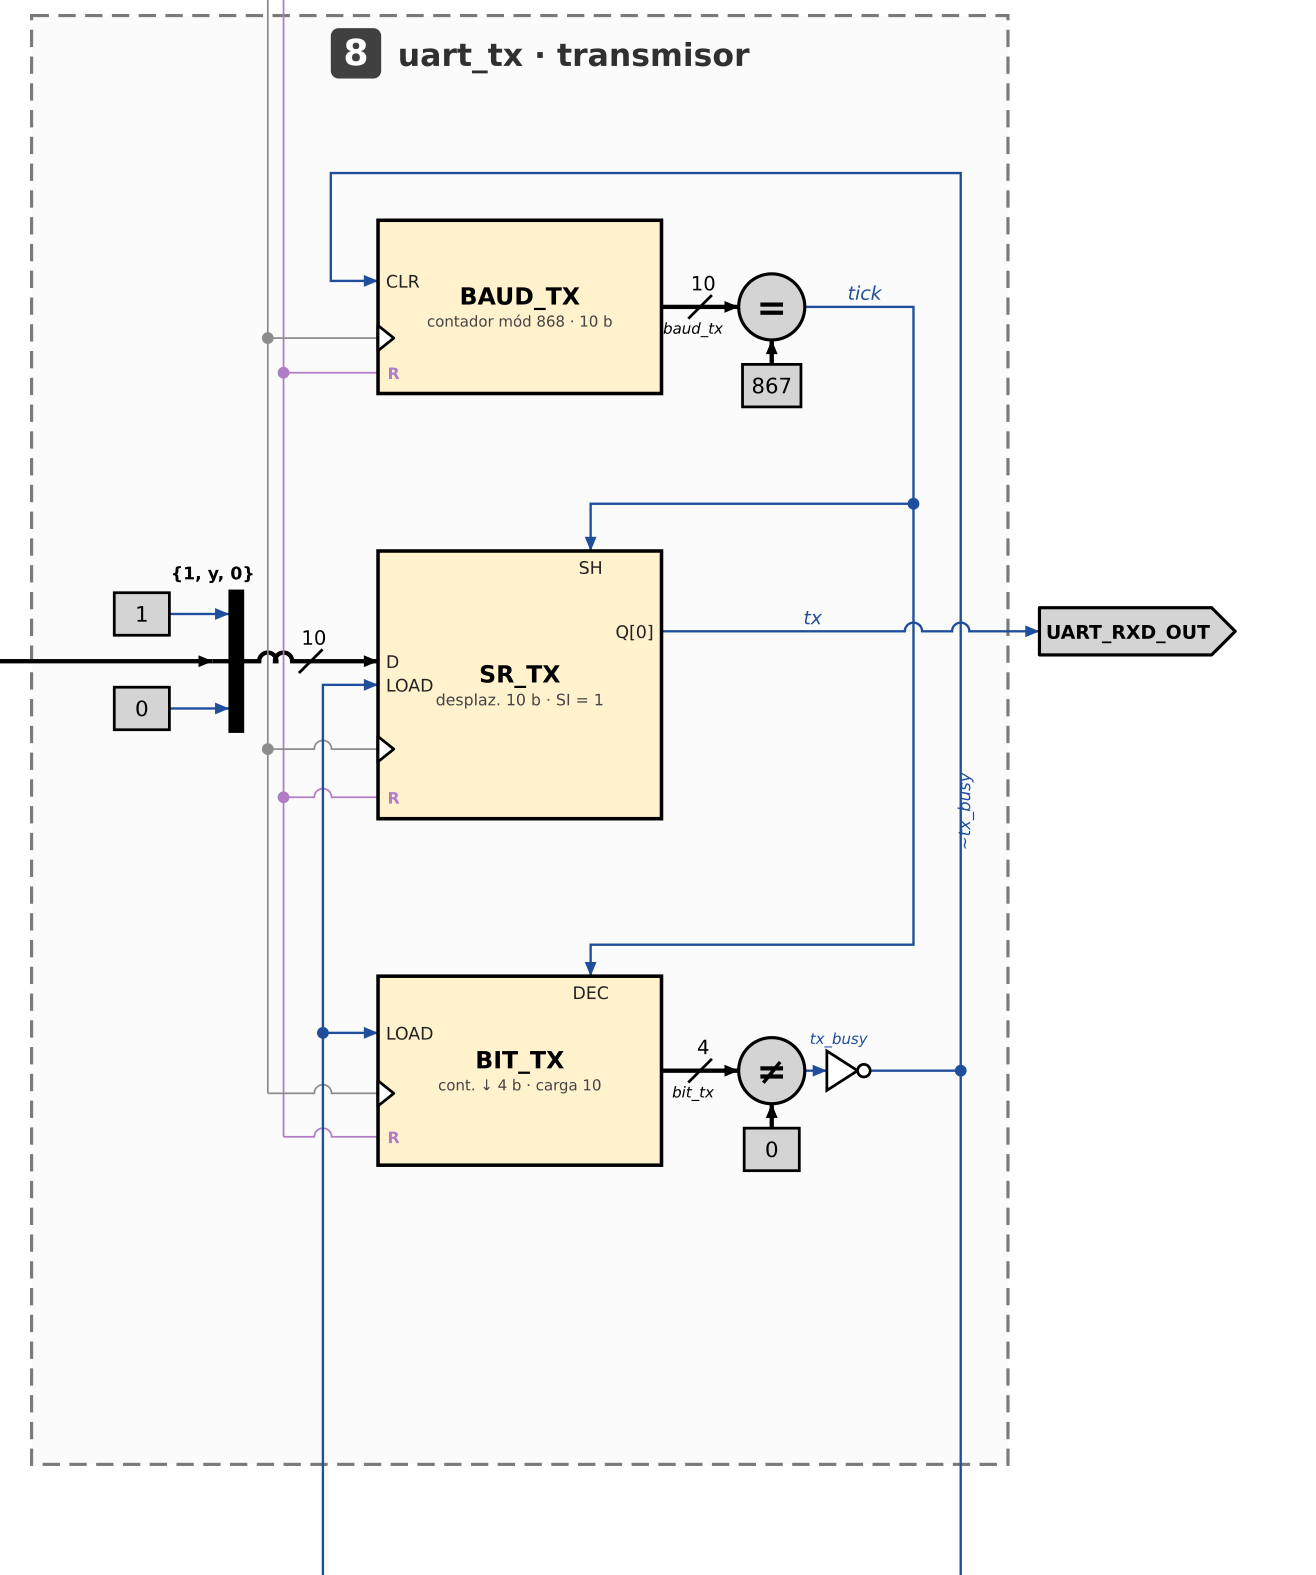
\includegraphics[width=0.55\linewidth]{img/blk8.png}\end{center}

\textbf{Hardware.}
\begin{itemize}
\item \textbf{SR\_TX} (10\,b, carga paralela y desplazamiento): con \sig{tx\_start} carga \{1, \bus{y}, 0\} $=$ \{parada, dato, inicio\}; con \sig{tick} se corre a la derecha metiendo un 1. La línea es \bus{SR\_TX[0]}: primero sale el 0 de inicio, luego el LSB del dato… y al final el registro queda lleno de unos (línea en reposo) sin necesidad de otro multiplexor.
\item \textbf{BIT\_TX} (4\,b, descendente): carga 10 con \sig{tx\_start} y resta 1 con cada \sig{tick}. \sig{tx\_busy} $=$ (\bus{bit\_tx} $\neq 0$).
\item \textbf{BAUD\_TX}: contador módulo 868 que se borra mientras \sig{tx\_busy} = 0; \sig{tick} $=$ (\bus{baud\_tx} $= 867$) marca el final de cada bit.
\end{itemize}
El transmisor no se protege contra un \sig{tx\_start} con \sig{tx\_busy} = 1 porque la unidad de control nunca lo produce: \sig{go} $=$ \sig{at11} $\cdot\,\overline{\sig{tx\_busy}}$.

\textbf{Verificación (\texttt{tb\_uart\_tx}, 868 ciclos por bit):} la línea se compara \emph{ciclo a ciclo} con la forma ideal (2,5 millones de comparaciones) para los 256 valores y 32 bytes con pausas; \sig{tx\_busy} dura exactamente 8\,680 ciclos. PASS.

\subsection{Bloque 9 — \texorpdfstring{\texttt{ctrl}}{ctrl}: unidad de control}
\begin{center}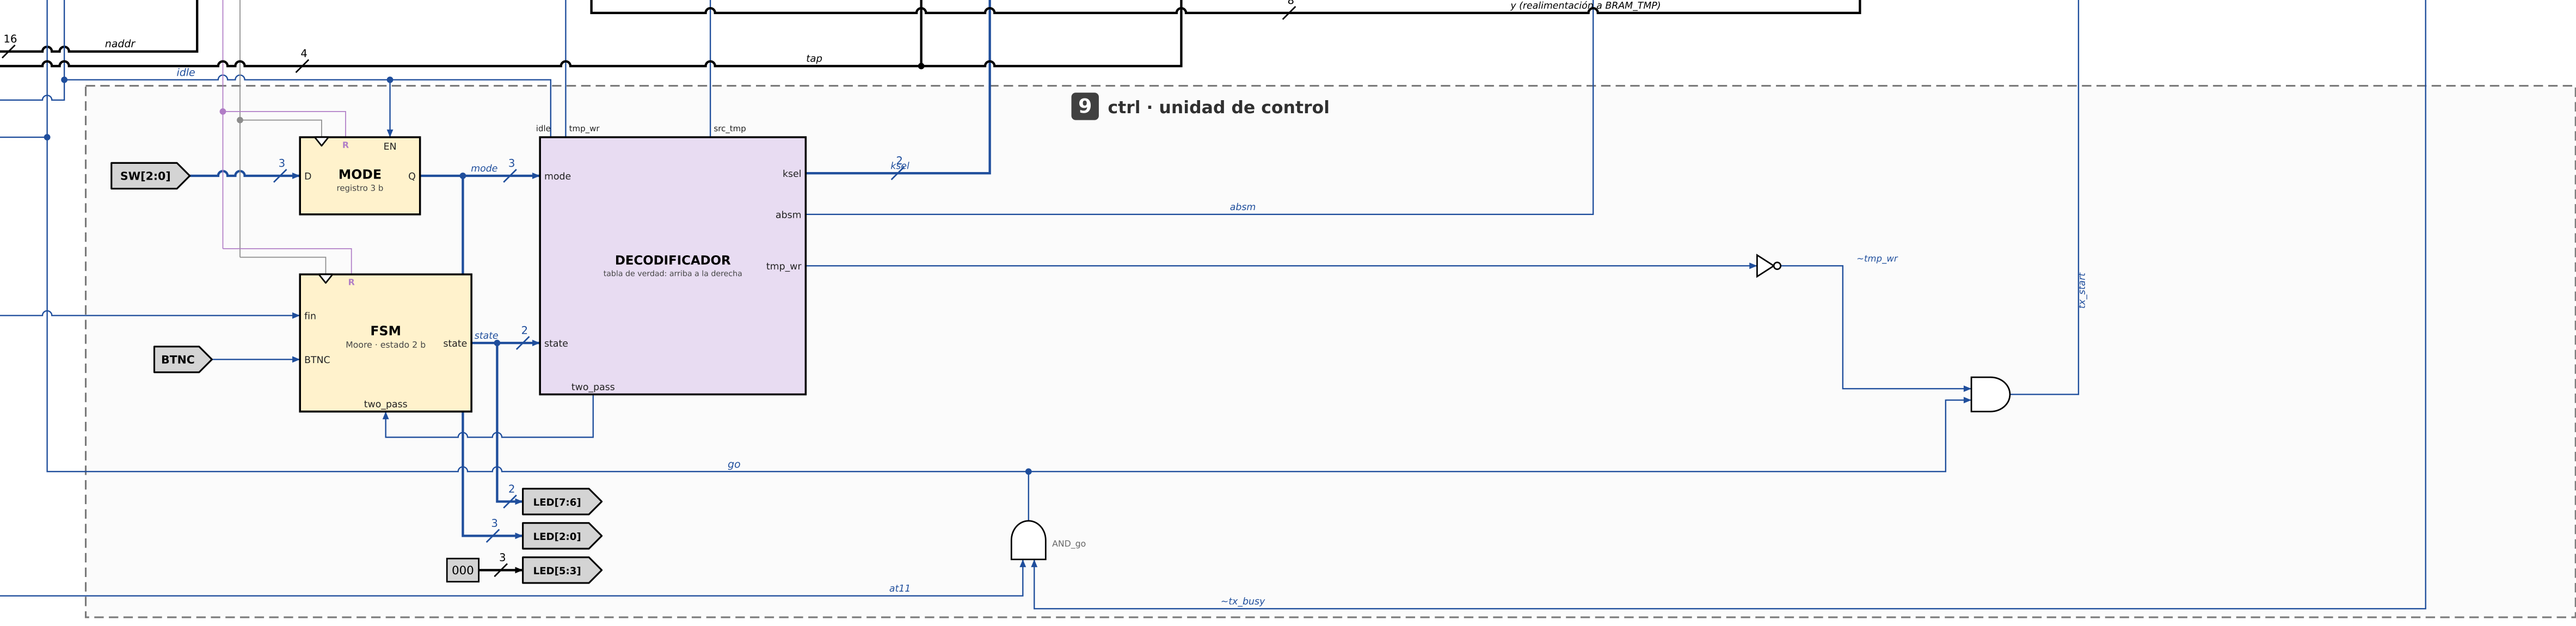
\includegraphics[width=\linewidth]{img/blk9.png}\end{center}

\textbf{FSM de Moore} con estado de 2\,bits (IDLE = 00, P1 = 01, P2 = 10):
\[
\text{IDLE} \xrightarrow{\ fin\, +\, BTNC\ } \text{P1},\qquad
\text{P1} \xrightarrow{\ fin \cdot two\_pass\ } \text{P2},\qquad
\text{P1} \xrightarrow{\ fin \cdot \overline{two\_pass}\ } \text{IDLE},\qquad
\text{P2} \xrightarrow{\ fin\ } \text{IDLE}.
\]
IDLE $\to$ P1 cambia solo el bit 0 del estado: \bus{BTNC}, que llega sin sincronizador ni antirrebote (D15, D16), afecta un único flip-flop de decisión; el atributo \texttt{fsm\_encoding = "none"} impide que Vivado cambie la codificación. Además, la FSM solo mira \bus{BTNC} en IDLE y no vuelve a IDLE antes de 4,27\,s, así que los rebotes no causan nada.

\textbf{MODE} (3\,b) copia \bus{SW[2:0]} mientras el estado es IDLE (EN $=$ \sig{idle}) y queda congelado en P1/P2: mover los switches durante el procesamiento no mezcla filtros.

\textbf{Decodificador} (combinacional; ver tabla T del esquemático):

\begin{center}
\small
\begin{tabular}{llcccccc}
\toprule
\textbf{state} & \textbf{MODE} & \textbf{ksel} & \textbf{absm} & \textbf{src\_tmp} & \textbf{tmp\_wr} & \textbf{idle} & \textbf{two\_pass} \\
\midrule
IDLE & x xx & — & — & 0 & 0 & 1 & — \\
P1 & 0 00 (G) & 00 & 0 & 0 & 0 & 0 & 0 \\
P1 & 0 01 (L) & 01 & 1 & 0 & 0 & 0 & 0 \\
P1 & 0 10 (LoG) & 00 & 0 & 0 & 1 & 0 & 1 \\
P1 & 0 11 (US) & 11 & 0 & 0 & 0 & 0 & 0 \\
P1 & 1 xx (bypass) & 10 & 0 & 0 & 0 & 0 & 0 \\
P2 & x xx & 01 & 1 & 1 & 0 & 0 & 1 \\
\bottomrule
\end{tabular}
\end{center}

\textbf{Compuertas de control} (las marcadas ctrl están dibujadas junto a su uso):
\[
\begin{aligned}
wr\_in &= rx\_valid \cdot idle && \text{(solo se recibe en IDLE; bytes que lleguen procesando se ignoran)}\\
cnt\_en &= wr\_in + go && \text{(avanza la posición)}\\
go &= at11 \cdot \overline{tx\_busy} && \text{(byte listo y UART libre)}\\
tap\_en &= \overline{at11 + idle} && \text{(TAP cuenta hasta 11, no en IDLE)}\\
tx\_start &= go \cdot \overline{tmp\_wr} && \text{(enviar, salvo en la 1.ª pasada del LoG)}\\
we\_tmp &= tmp\_wr && \text{(BRAM\_TMP se escribe en toda la 1.ª pasada del LoG)}
\end{aligned}
\]
En la primera pasada del LoG no se transmite, así que \sig{tx\_busy} = 0 y \sig{go} $=$ \sig{at11}: el mismo \sig{go} sirve para las dos clases de pasada.

\textbf{Verificación (\texttt{tb\_ctrl}):} los 8 valores de \bus{SW[2:0]}, arranque con \sig{fin} y con \bus{BTNC}, \bus{BTNC} y switches ignorados en P1/P2, MODE congelado, la segunda pasada solo en LoG y todas las salidas contra la tabla. PASS.

% =====================================================================
\section{Recorrido de un byte, ciclo a ciclo}

Este ejemplo sale de la simulación del sistema completo (imagen de 4\,×\,4, Gaussiano). Se calcula el canal R del píxel (0, 0), que está en una esquina: los vecinos de arriba y de la izquierda no existen y se replican.
Los valores de la imagen en el canal R son: $(0,0) = 17$, $(0,1) = 176$, $(1,0) = 141$, $(1,1) = 44$.

\begin{center}
\footnotesize
\begin{tabularx}{\linewidth}{ccccccccX}
\toprule
\textbf{tap} & \textbf{vecino} & \textbf{naddr} & \textbf{pix} & \textbf{w} & \textbf{pix\_q·w\_q} & \textbf{acc al final} & \textbf{y} & \textbf{qué pasa} \\
\midrule
0 & $(-1,-1)$ & (0, 0) & — & 0 & — & 0 & & se borra ACC (\bus{tap} = 0) \\
1 & $(-1,\ 0)$ & (0, 0) & 17 & 1 & $177 \cdot 0$ & 0 & & sale el vecino del tap 0 \\
2 & $(-1,+1)$ & (0, 1) & 17 & 2 & $17 \cdot 1$ & 17 & & primer término \\
3 & $(0,-1)$ & (0, 0) & 176 & 1 & $17 \cdot 2$ & 51 & & \\
4 & $(0,\ 0)$ & (0, 0) & 17 & 2 & $176 \cdot 1$ & 227 & & \\
5 & $(0,+1)$ & (0, 1) & 17 & 4 & $17 \cdot 2$ & 261 & & \\
6 & $(+1,-1)$ & (1, 0) & 176 & 2 & $17 \cdot 4$ & 329 & & centro (peso 4) \\
7 & $(+1,\ 0)$ & (1, 0) & 141 & 1 & $176 \cdot 2$ & 681 & & \\
8 & $(+1,+1)$ & (1, 1) & 141 & 2 & $141 \cdot 1$ & 822 & & \\
9 & centro & (0, 0) & 44 & 1 & $141 \cdot 2$ & 1104 & & \\
10 & centro & (0, 0) & 17 & 0 & $44 \cdot 1$ & 1148 & & último término \\
11 & centro & (0, 0) & 17 & 0 & $17 \cdot 0$ & 1148 & 71 & \sig{at11}, \sig{go}, \sig{tx\_start} \\
\bottomrule
\end{tabularx}
\end{center}
La columna \textbf{vecino} es el desplazamiento pedido en ese tap y \textbf{naddr} muestra (fila, columna) del vecino ya ajustado al borde; el canal es 0 en todos los ciclos. \textbf{pix} es el byte que sale de la BRAM en ese ciclo (el pedido en el tap anterior) y \textbf{w} el peso de la ROM\_W. La columna \textbf{pix\_q · w\_q} es el producto que entra al ACC en ese ciclo: el píxel y el peso que salieron un ciclo antes y quedaron en REG\_PIX y REG\_W. En el tap 1, REG\_PIX todavía tiene un valor viejo (177, del byte anterior), pero el peso registrado es ROM\_W[0] $= 0$, así que no suma nada.

Resultado: $y = \lfloor 1148/16 \rfloor = 71$. La figura~\ref{fig:wmac} muestra exactamente esta secuencia: el siguiente byte (canal G del mismo píxel) se calcula en los 12 ciclos siguientes ($acc = 1996 \Rightarrow y = 124$) y espera en el tap 11 porque la UART está ocupada con el primero.

\begin{figure}[H]
\centering
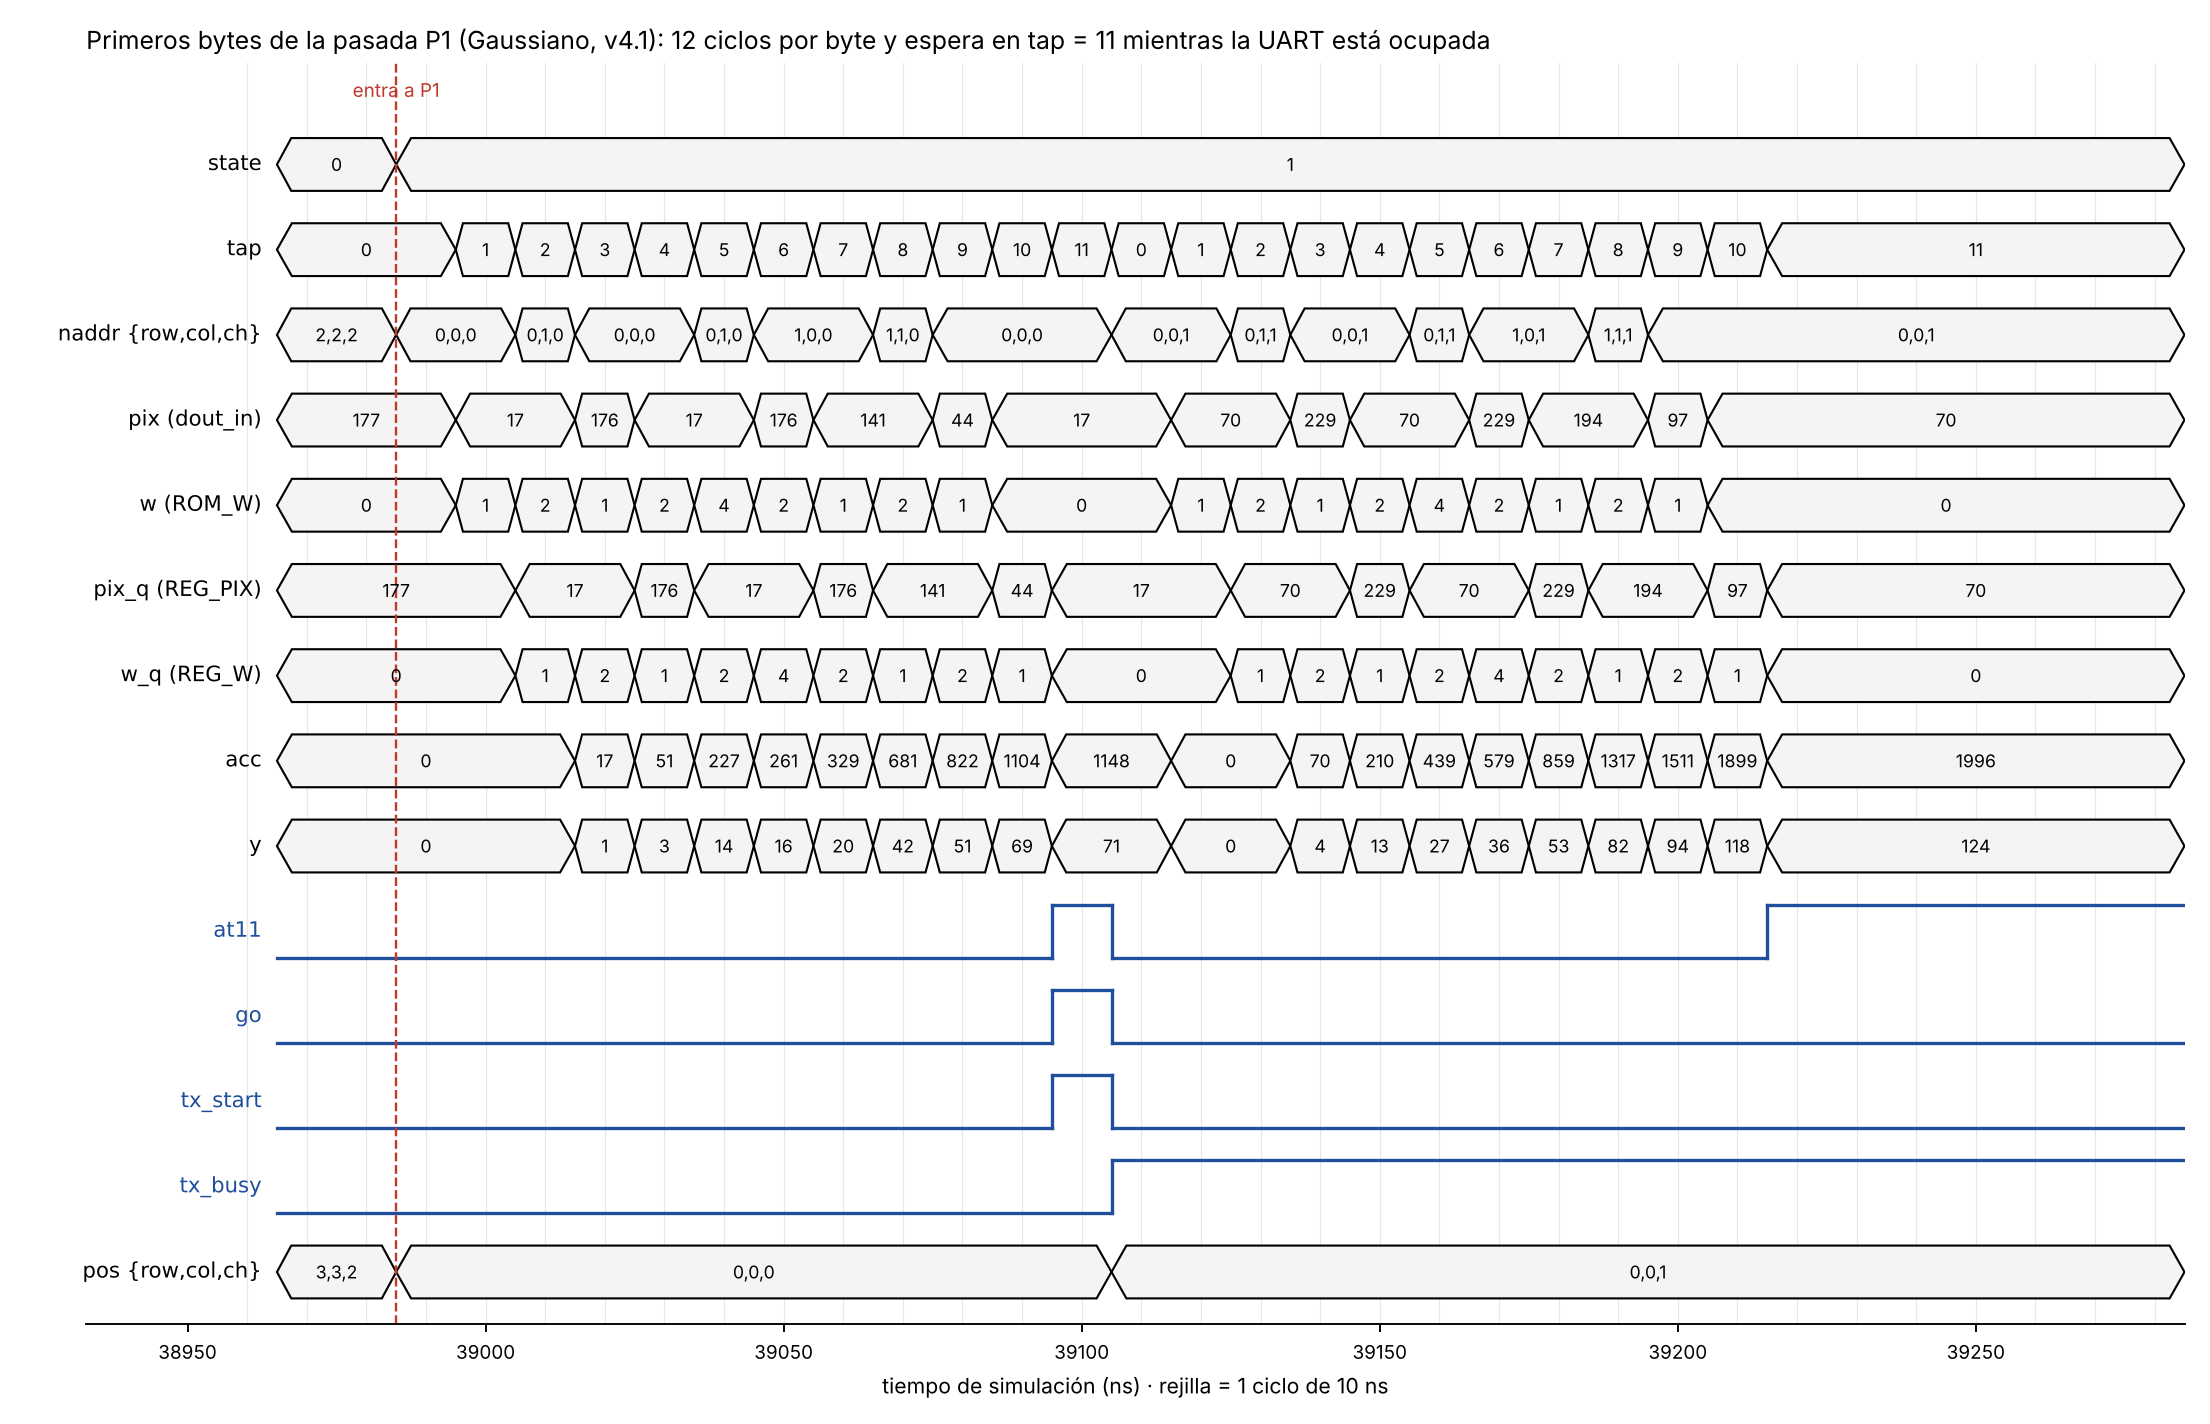
\includegraphics[width=\linewidth]{img/wave_mac.png}
\caption{Simulación del sistema (v4.1): primeros bytes de la pasada P1. \bus{pix\_q} y \bus{w\_q} repiten \bus{pix} y \bus{w} un ciclo después; el ACC acumula 17, 51, 227, … 1148 y en el tap 11 se entrega $y = 71$.}
\label{fig:wmac}
\end{figure}

\begin{figure}[H]
\centering
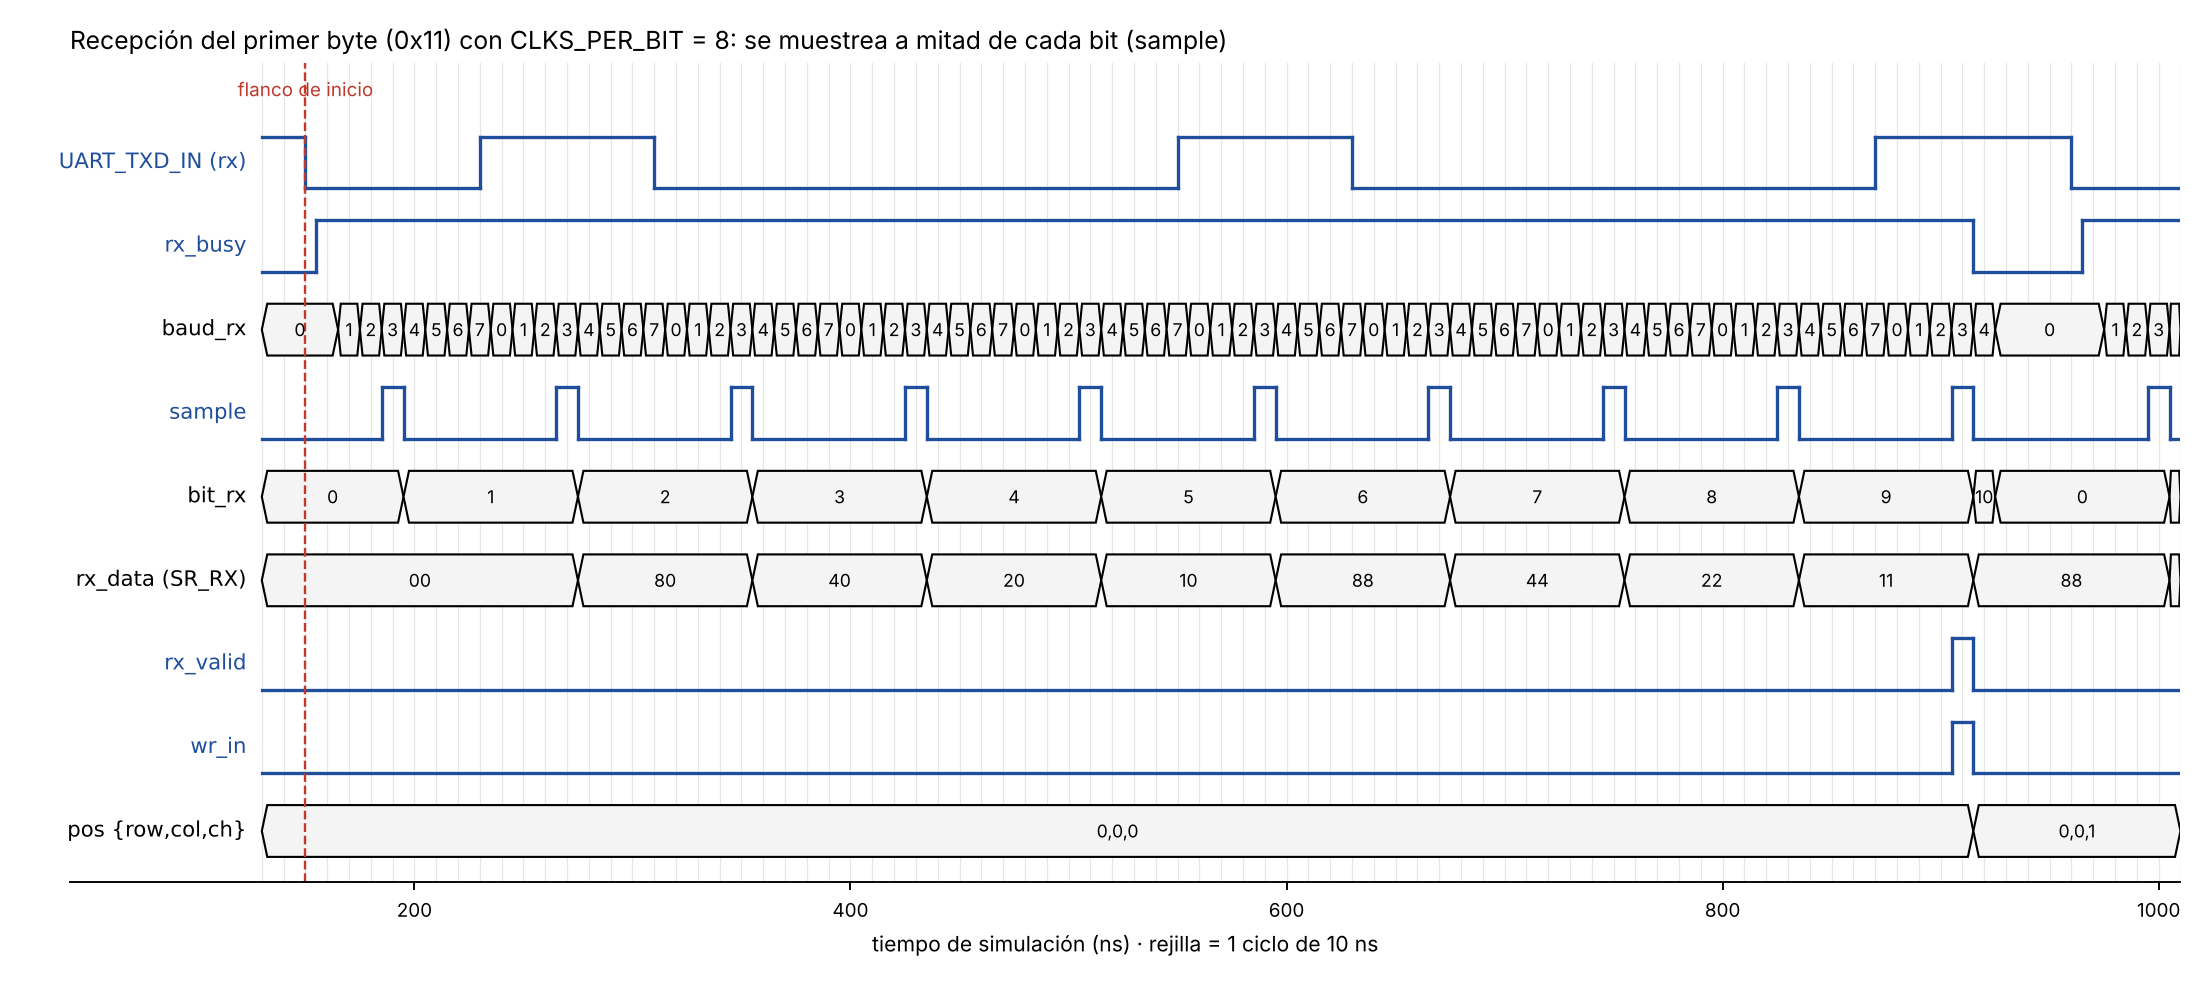
\includegraphics[width=\linewidth]{img/wave_rx.png}
\caption{Recepción del byte 0x11 (simulación con 8 ciclos por bit en lugar de 868, D14): se muestrea a mitad de cada bit; en la muestra 9 sale \sig{rx\_valid} con \bus{rx\_data} = 0x11 y se escribe en la posición (0, 0, 0).}
\end{figure}

% =====================================================================
\section{Anchos de bus: de dónde salen}

\begin{itemize}
\item \textbf{Producto (15\,b).} El peso de mayor magnitud es $-64$ y el píxel máximo 255: $|w\cdot x| \le 64 \cdot 255 = 16\,320 < 2^{14} = 16\,384$. Con signo hacen falta $14 + 1 = 15$ bits (el multiplicador produce 17, los dos bits altos son solo signo).
\item \textbf{ACC (15\,b).} Hay que acotar la suma de los 9 términos para cada kernel:
\[
\begin{array}{lll}
G: & 0 \le acc \le 16\cdot255 = 4\,080 \\
16L: & -64\cdot255 = -16\,320 \le acc \le 4\cdot16\cdot255 = 16\,320 \\
16\delta: & 0 \le acc \le 4\,080 \\
U: & -12\cdot255 = -3\,060 \le acc \le 28\cdot255 = 7\,140
\end{array}
\]
Todas caben en $[-2^{14}, 2^{14}-1] = [-16\,384, 16\,383]$: 15 bits con signo. Las sumas parciales también, porque nunca superan la suma de los términos positivos ni bajan de la de los negativos.
\item \textbf{$s$ (11\,b).} $acc/16 \in [-1\,020, 1\,020]$ necesita 11\,bits con signo.
\item \textbf{$v$ (11\,b).} $|s| \le 1\,020$; se usan 11\,bits para que el bloque sea correcto incluso con el valor extremo $-16\,384$ (ver bloque 7).
\item \textbf{Dirección (16\,b).} 7 de fila + 7 de columna + 2 de canal.
\item \textbf{Contadores de baudios (10\,b).} $868 < 2^{10}$. \textbf{BIT\_RX y BIT\_TX (4\,b):} cuentan hasta 9 y 10. \textbf{TAP (4\,b):} hasta 11. \textbf{REG\_PIX y REG\_W (8\,b):} el mismo ancho que \bus{pix} y \bus{w}.
\end{itemize}

% =====================================================================
\section{Verificación: qué se simuló y qué salió}

Todo se simuló con Icarus Verilog 12 (\texttt{iverilog -g2012}). Cada testbench se comprueba solo: compara contra un modelo escrito en el propio testbench y termina con PASS o FAIL. El modelo de referencia de los filtros vive \emph{solo} en el testbench, no en el sistema (R-F01). El RTL además pasa \texttt{verilator --lint-only -Wall} sin advertencias. En \textbf{Vivado 2025.2} se corrió el testbench del sistema en el simulador xsim (4\,441 verificaciones, 0 errores, PASS: el mismo resultado que en Icarus) y el diseño se sintetizó, implementó y generó el bitstream (sección~\ref{sec:tiempos}). Después del cambio a v4.1 se volvieron a correr los 10 testbenches y la imagen completa.

\begin{center}
\small
\begin{tabularx}{\linewidth}{>{\ttfamily}l r >{\raggedright\arraybackslash}X c}
\toprule
\normalfont\textbf{Testbench} & \textbf{Compar.} & \textbf{Casos límite cubiertos} & \textbf{Res.} \\
\midrule
tb\_uart\_rx & 397 & 256 valores seguidos, pausas aleatorias, $\pm3$\,\% de baudios, punto de muestreo, reposo, reset a mitad de byte & PASS \\
tb\_uart\_tx & 2\,510\,598 & línea comparada ciclo a ciclo, 256 valores, envío seguido, duración de \texttt{busy} & PASS \\
tb\_noise\_gen & 613\,697 & período del LFSR, aciertos exactos por nivel, modelo ciclo a ciclo, decisión común por píxel & PASS \\
tb\_pos\_counter & 393\,298 & dos tamaños, enable aleatorio, vueltas, \texttt{fin} & PASS \\
tb\_bram\_sdp & 431\,081 & latencia, extremos, colisión, barrido completo & PASS \\
tb\_tap\_seq & 221\,170 & exhaustivo: 16\,384 posiciones × 12 taps, espera, \texttt{go}, IDLE & PASS \\
tb\_conv\_mac & 36\,073 & 4 kernels, extremos y aleatorios, retención en tap 11, rango del ACC & PASS \\
tb\_post\_proc & 65\,536 & exhaustivo: todos los valores del ACC × \texttt{absm} & PASS \\
tb\_ctrl & 157 & 8 modos, arranques, BTNC ignorado, MODE congelado, tabla & PASS \\
tb\_image\_proc\_top 8×8 & 4\,441 & sistema por los pines: G, L, LoG, US, bypass, extremos, 3 niveles de ruido, BRAM\_TMP, LEDs, bytes ajenos durante el proceso, BTNC sostenido; también en Vivado xsim & PASS \\
tb\_image\_proc\_top 128×128 & 491\,529 & imagen real: los 5 modos y ruido; 49\,152/49\,152 bytes iguales al modelo en cada uno & PASS \\
\bottomrule
\end{tabularx}
\end{center}

\textbf{Imagen completa de 128\,×\,128.} La figura~\ref{fig:gal} muestra las salidas \emph{de la simulación RTL} (no de Python): cada una coincide byte a byte con el modelo. Con ruido de nivel 2 se afectaron 2\,105 de 16\,384 píxeles (12,85\,\%; esperado 12,5\,\%). El patrón de ruido no es el mismo de la v4 porque el LFSR corre libre y la v4.1 tarda un ciclo más por byte; las salidas de los cinco filtros sin ruido sí son idénticas byte a byte a las de v4. Entre dos bytes de salida pasan siempre $10 \times 8 + 1 = 81$ ciclos en la simulación (8 ciclos por bit), lo que en la tarjeta son $8\,681$ ciclos.

\begin{figure}[H]
\centering
\setlength{\tabcolsep}{2pt}
\begin{tabular}{cccc}

\includegraphics[width=0.235\linewidth]{img/sim_in_x3.png} &

\includegraphics[width=0.235\linewidth]{img/sim_G_x3.png} &
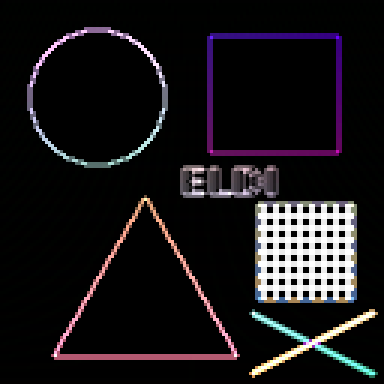
\includegraphics[width=0.235\linewidth]{img/sim_L_x3.png} &
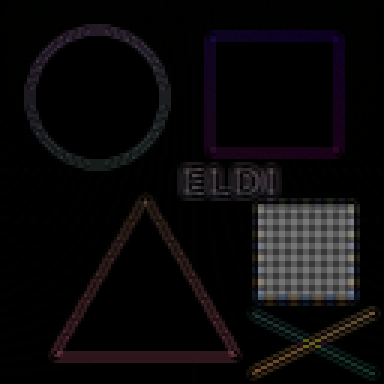
\includegraphics[width=0.235\linewidth]{img/sim_LoG_x3.png} \\
\small entrada / bypass & \small Gaussiano & \small Laplaciano $|L|$ & \small LoG \\[3pt]

\includegraphics[width=0.235\linewidth]{img/sim_US_x3.png} &
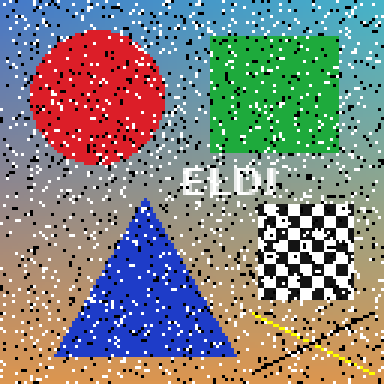
\includegraphics[width=0.235\linewidth]{img/sim_NOISE_x3.png} &
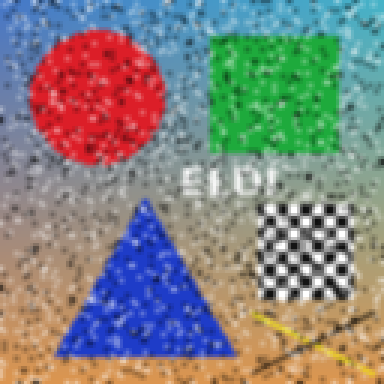
\includegraphics[width=0.235\linewidth]{img/sim_NG_x3.png} &

\includegraphics[width=0.235\linewidth]{img/sim_LoGx4_x3.png} \\
\small Unsharp & \small ruido 12,5\,\% (bypass) & \small Gaussiano sobre ruido & \small LoG (×4 solo para verlo) \\
\end{tabular}
\caption{Salidas de la simulación RTL del sistema completo con la imagen de prueba de 128\,×\,128.}
\label{fig:gal}
\end{figure}

\begin{ojo}
\textbf{El LoG sale oscuro y es correcto.} El Gaussiano suaviza los bordes antes de derivar, así que los valores del Laplaciano son pequeños (la última imagen está multiplicada por 4 \emph{solo} en el documento para que se vea). Si en la sustentación se quiere más contraste, una opción sería escalar el resultado del LoG; hoy no se hace porque ningún requisito lo pide y cambiaría la normalización.
\end{ojo}

% =====================================================================
\section{Implementación en Vivado 2025.2 y cierre de tiempos (v4.1)}
\label{sec:tiempos}

\subsection{Qué se hizo en Vivado}
{\sloppy Proyecto \texttt{FINAL} con la parte \texttt{xc7a100tcsg324-1} (XC7A100T, encapsulado CSG324, grado de velocidad $-1$), las fuentes de \texttt{rtl/}, los testbenches como fuentes de simulación y la XDC \texttt{nexys\_a7\_100t.xdc}. La XDC se generó descomentando las líneas del archivo maestro oficial de Digilent (\texttt{Nexys-A7-100T-Master.xdc}): ningún pin se escribió a mano. Se corrió la simulación del sistema en xsim, la síntesis, la implementación y el bitstream.\par}

\subsection{El problema: la v4 no cumplía los tiempos}
En un circuito síncrono, el dato que sale de un registro debe atravesar la lógica y llegar al siguiente registro antes del próximo flanco de reloj. Es la restricción de \emph{setup} de la presentación 8 (diapositiva 127), y con el desfase de reloj (\emph{skew}, diapositivas 133–134):
\[
T_c \;\ge\; t_{pcq} + t_{pd} + t_{setup} + t_{skew}, \qquad T_c = \frac{1}{100\ \text{MHz}} = 10\ \text{ns}.
\]
Vivado calcula para cada camino el margen (\emph{slack}) $=$ tiempo disponible $-$ tiempo de llegada. El peor margen se llama \textbf{WNS} (\emph{worst negative slack}). Si es negativo, el registro de destino puede capturar un valor que todavía está cambiando: la simulación (que no tiene retardos) pasa, pero la tarjeta puede dar resultados erróneos de forma aleatoria.

El reporte de la v4 dio \textbf{WNS $= -1{,}669$\,ns}, con 8 de 1\,353 puntos de llegada (\emph{endpoints}) fallando (TNS $= -8{,}465$\,ns). El peor camino iba de BRAM\_IN al bit 14 del ACC:

\begin{center}
\small
\begin{tabularx}{\linewidth}{>{\raggedright\arraybackslash}X r}
\toprule
\textbf{Tramo del camino crítico (v4)} & \textbf{Retardo} \\
\midrule
Lectura de BRAM\_IN: reloj $\to$ salida, a través de dos RAMB36 en cascada (65\,536 × 8 se arma con bloques de 32\,K × 1) & 3,36\,ns \\
Ruteo desde la BRAM hasta la primera LUT & 1,69\,ns \\
MUX\_SRC, multiplicador y sumador hasta la entrada D del ACC (5 LUT y 5 bloques de acarreo CARRY4), con su ruteo & 6,30\,ns \\
\midrule
\textbf{Total del camino de datos} (11 niveles de lógica; 6,59\,ns de lógica y 4,76\,ns de ruteo) & \textbf{11,35\,ns} \\
Tiempo disponible (10\,ns, menos el desfase de reloj de 0,34\,ns y la incertidumbre de 0,035\,ns) & $\approx$ 9,68\,ns \\
\bottomrule
\end{tabularx}
\end{center}

\subsection{Alternativas que se consideraron}
\begin{center}
\small
\begin{tabularx}{\linewidth}{>{\raggedright\arraybackslash}p{3.6cm}>{\raggedright\arraybackslash}X>{\raggedright\arraybackslash}X}
\toprule
\textbf{Opción} & \textbf{A favor} & \textbf{En contra} \\
\midrule
Bajar el reloj (por ejemplo a 50\,MHz) & No toca el camino de datos & Requiere un MMCM o PLL (no visto en el curso) o un divisor de reloj (mala práctica en FPGA); cambia \texttt{CLKS\_PER\_BIT} y el análisis de la UART \\
Forzar el multiplicador a un DSP48 & El DSP multiplica más rápido que las LUT & Solo la BRAM y su ruteo ya gastan unos 5\,ns; el margen quedaría muy justo y dependería de cómo coloque Vivado los bloques \\
\textbf{Registro de segmentación} entre la BRAM y el multiplicador (\textbf{elegida}) & Parte el camino en dos tramos cortos; es la técnica de las presentaciones 8 (diapositiva 60: las dos estructuras síncronas típicas son las FSM y los \emph{pipelines}) y 10 (procesador segmentado) & 16 flip-flops más y un ciclo más por byte \\
\bottomrule
\end{tabularx}
\end{center}

\subsection{La solución: REG\_PIX y REG\_W}
Se agregan dos registros de 8\,bits en el bloque 6: \textbf{REG\_PIX} guarda el píxel que sale de MUX\_SRC y \textbf{REG\_W} guarda el peso que sale de ROM\_W. El camino largo queda partido en dos:
\[
\underbrace{\text{BRAM} \to \text{MUX\_SRC} \to \text{REG\_PIX}}_{\text{tramo 1}}
\qquad\text{y}\qquad
\underbrace{\text{REG\_PIX, REG\_W} \to \times \to + \to \text{ACC}}_{\text{tramo 2}} .
\]
\begin{itemize}
\item \textbf{El peso también se registra} para que siga alineado con su píxel: la fila $t$ de la ROM\_W es el peso del píxel que sale de la BRAM en el tap $t$; ambos se guardan al final del tap $t$ y se multiplican en el tap $t+1$.
\item \textbf{Cada producto entra al ACC un tap después.} El primero (vecino pedido en el tap 0) entra en el tap 2 y el último (vecino del tap 8) en el tap 10, así que el resultado está listo en el \textbf{tap 11}. Por eso TAP ahora cuenta 0…11, el comparador pasa de $=10$ a $=11$ (señal \sig{at11}), la ROM\_OFF tiene la fila 11 (centro) y la ROM\_W tiene la fila 11 con peso 0.
\item \textbf{El borrado del ACC no cambia.} Sigue siendo en el tap 0, porque en el tap 1 el peso registrado es ROM\_W[0] $= 0$ y el primer término que entra vale 0.
\item \textbf{Costo:} 12 ciclos por byte en lugar de 11. Una pasada sin UART tarda $12 \times 49\,152 = 589\,824$ ciclos $\approx 5{,}9$\,ms (antes 5,4\,ms), algo invisible frente a los 4,27\,s de la UART. La UART sigue mandando un byte cada 8\,681 ciclos.
\end{itemize}

\subsection{Resultado en Vivado}
\begin{center}
\small
\begin{tabular}{lrr}
\toprule
\textbf{Diseño implementado} & \textbf{v4} & \textbf{v4.1} \\
\midrule
WNS (margen de \emph{setup} del peor camino) & $-1{,}669$\,ns & $\mathbf{+2{,}112}$\,ns \\
TNS (suma de márgenes negativos) & $-8{,}465$\,ns & 0 \\
Puntos de llegada que no cumplen & 8 & 0 \\
WHS (margen de \emph{hold} del peor camino) & $+0{,}152$\,ns & $+0{,}116$\,ns \\
LUT & 305 & 313 \\
Flip-flops & 120 & 137 \\
Bloques RAMB36 & 32 & 32 \\
DSP48 & 0 & 0 \\
Pines (IOB) & 18 & 18 \\
\bottomrule
\end{tabular}
\end{center}
\begin{itemize}
\item \textbf{Todos los tiempos se cumplen} (\emph{All user specified timing constraints are met}). El nuevo peor camino ya no es el MAC: va del registro MODE a la habilitación de BRAM\_TMP (7,24\,ns, de los cuales 6,66\,ns son ruteo, porque esa señal tiene que llegar a los 16 bloques de BRAM\_TMP) y le sobran 2,11\,ns.
\item \textbf{Flip-flops: +17.} 16 son REG\_PIX y REG\_W; la diferencia restante sale de cómo Vivado optimizó el resto del circuito.
\item \textbf{Las cifras reales difieren de la estimación de Yosys} (1 DSP48, 91 FF, unos 176 LUT): Vivado hizo el multiplicador con LUT y no con un DSP. El reporte que vale para el proyecto es el de Vivado.
\item \textbf{Verificación después del cambio:} los 10 testbenches pasan (\texttt{tb\_tap\_seq} ahora revisa 12 taps y \texttt{tb\_conv\_mac} revisa el resultado en el tap 11), la imagen completa de 128\,×\,128 da 491\,529 verificaciones sin errores y las salidas de los cinco filtros son idénticas byte a byte a las de v4.
\end{itemize}

% =====================================================================
\section{Trazabilidad de requisitos}

\begin{center}
\small
\begin{tabularx}{\linewidth}{l>{\raggedright\arraybackslash}X>{\raggedright\arraybackslash}X}
\toprule
\textbf{Req.} & \textbf{Dónde se cumple} & \textbf{Evidencia} \\
\midrule
R-P1 & Bloques 5, 6, 7 (G y L individuales; LoG = G luego L en dos pasadas; Unsharp = $2I - G$), imagen a color (cada canal) & \texttt{tb\_conv\_mac}, \texttt{tb\_post\_proc}, sistema 128\,×\,128 \\
R-P2 & Bloques 1 y 8: UART 8N1 a 115\,200\,Bd sobre el puente USB-UART & \texttt{tb\_uart\_rx}, \texttt{tb\_uart\_tx}, sistema por los pines \\
R-P3 & \texttt{SW[2:0]} $\to$ MODE $\to$ decodificador; \texttt{SW[4:3]} $\to$ ruido & \texttt{tb\_ctrl}, sistema \\
R-P4 & Bloque 2: ruido en la FPGA & \texttt{tb\_noise\_gen}, sistema (3 niveles) \\
R-F01 & Python solo envía, recibe y muestra; toda la matemática en la FPGA & arquitectura; el modelo de referencia vive solo en los testbenches \\
R-G03 & Un testbench autoverificable por módulo + sistema & 10 testbenches PASS en Icarus; el del sistema también en Vivado xsim \\
R-G04 & Extras: bypass, LEDs de modo y estado & sistema \\
R-G06 & Esquemático detallado: memorias, FSM, registros, sumador, multiplicador, shifter, MUX, decodificador, contadores, FF y anchos de bus & \texttt{esquematico\_v4\_1.pdf} \\
\bottomrule
\end{tabularx}
\end{center}

% =====================================================================
\section{Limitaciones, riesgos y pendientes}
\begin{itemize}
\item \textbf{Sin sincronizadores (D15).} Funciona con la justificación de un solo FF de decisión, pero es una decisión discutible y está entre las preguntas abiertas al profesor. \bus{SW[2:0]} sí llega a 3 FF (MODE); como los switches no se mueven al pulsar \bus{BTNC}, el riesgo es despreciable.
\item \textbf{Un byte perdido desalinea la imagen (D17).} No hay cabecera; se recupera con \bus{CPU\_RESETN} y reenviando. El procedimiento correcto es: detener el envío, pulsar reset y volver a enviar (si se resetea a mitad de un byte, el resto de ese byte puede leerse como un byte basura).
\item \textbf{LoG en dos pasadas.} Sigue abierta la pregunta al profesor sobre el kernel único de 5\,×\,5. Si lo acepta, se elimina BRAM\_TMP, MUX\_SRC y el estado P2; mientras tanto la versión en dos pasadas es la que cumple sin duda ``combinado'' (R-P1).
\item \textbf{Lo que falta probar:} la tarjeta (programar el bitstream y enviar una imagen real con el script de Python) y los testbenches de cada módulo en xsim (en Vivado solo se corrió el del sistema). La síntesis, la implementación y los tiempos a 100\,MHz ya se comprobaron en Vivado 2025.2 (sección~\ref{sec:tiempos}).
\item \textbf{Pines.} El RTL usa los nombres del archivo maestro de Digilent para la Nexys A7-100T (\texttt{CLK100MHZ}, \texttt{CPU\_RESETN}, \texttt{UART\_TXD\_IN}, \texttt{UART\_RXD\_OUT}, \texttt{SW}, \texttt{BTNC}, \texttt{LED}). La XDC del proyecto (\texttt{nexys\_a7\_100t.xdc}) se generó descomentando esas líneas del archivo oficial; según Digilent, el mismo archivo sirve para la Nexys 4 DDR. Si la tarjeta fuera la Nexys 4 \emph{original}, hay que usar \texttt{nexys4\_original.xdc}, porque los switches, los LED y el botón central van en otros pines.
\item \textbf{Código anterior.} La v4 se escribió desde cero a partir de las decisiones de diseño (\texttt{docs/03\_decisiones.md}). Los módulos de v3 (\texttt{pixel\_assembler}, \texttt{addr\_gen}, \texttt{conv\_engine}, \texttt{conv\_lane}, \texttt{unsharp\_lane}, \texttt{tx\_path}, \texttt{ctrl\_fsm}) se reemplazan por los de v4; el protocolo con el PC no cambia.
\end{itemize}

% =====================================================================
\section{Preguntas para preparar la sustentación}
Las respuestas están en el anexo A.
\begin{enumerate}
\item ¿Por qué el receptor muestrea cuando \bus{baud\_rx} $= 433$ y no cuando vale 0? ¿Qué pasaría si el PC transmitiera un 3\,\% más lento?
\item En la simulación \bus{rx\_data} vale 0x80, 0x40, 0x20, … antes de llegar a 0x11. ¿Por qué? ¿Por qué no hace falta un registro aparte para guardar el byte?
\item ¿Por qué la ROM\_W está ``corrida un tap''? ¿Qué pasaría si la fila $t$ guardara el peso del vecino $t$?
\item Demuestre que el ACC necesita 15 bits. ¿Cuál kernel produce el extremo?
\item ¿Qué indica \bus{rsum[7]} y por qué basta un bit para detectar el borde?
\item Escriba el kernel del Unsharp a partir de $2I - G$ y explique por qué el centro vale 28.
\item Predicción: un vecindario con los 8 vecinos en 255 y el centro en 0. ¿Cuánto vale $y$ con el Laplaciano y con el Unsharp?
\item ¿Por qué se puede escribir BRAM\_TMP en todos los ciclos de la primera pasada del LoG sin dañar el resultado?
\item ¿Cuántos ciclos separan dos bytes de salida en la tarjeta? ¿Cuánto tarda en volver la imagen completa? ¿Y el cálculo sin la UART?
\item ¿Por qué el LFSR se congela durante los tres bytes de un píxel? ¿Qué pasaría si avanzara un paso por píxel?
\item ¿Qué pasa si se mueve un switch mientras la FPGA está procesando? ¿Y si llega un byte por la UART en ese momento?
\item ¿Por qué no hay sincronizador en \bus{BTNC} y por qué no rebota la FSM?
\item ¿Por qué la v4 no cumplía los tiempos a 100\,MHz aunque pasaba todas las simulaciones? ¿Qué hace la v4.1 y cuánto cuesta?
\end{enumerate}

\appendix
\section{Respuestas}
\begin{enumerate}
\item El contador se borra en el flanco de inicio, así que 433 cae en la mitad del bit, lo más lejos posible de los dos flancos. Con un 3\,\% de error, después de 9,5 bits el punto de muestreo se corre $9{,}5 \times 0{,}03 \approx 0{,}29$ bits: sigue dentro del bit (margen de $\pm0{,}5$). El testbench lo prueba con $+3$\,\% y $-3$\,\%.
\item SR\_RX se desplaza en cada muestra; tras las 9 primeras (inicio + 8 datos), el bit de inicio ya salió por la derecha y quedan los 8 datos en orden. \sig{rx\_valid} se activa en la muestra 9, antes de que el bit de parada entre al registro, y en ese mismo flanco el byte se escribe en BRAM\_IN: no hace falta otro registro.
\item Porque la BRAM entrega el dato un ciclo después de pedirlo. El peso debe acompañar al dato que llega, no a la dirección que sale. Sin el corrimiento, cada vecino se multiplicaría por el peso del siguiente. En v4.1 el peso y el píxel se registran juntos (REG\_W y REG\_PIX), así que siguen alineados.
\item Ver la sección 6: el Laplaciano ×16 llega a $\pm16\,320$, que necesita 15 bits con signo ($2^{14} = 16\,384$).
\item La suma $\{0,\text{fila}\} + dr$ está en $[-1, 128]$; en 8 bits, $-1 = 11111111_2$ y $128 = 10000000_2$ son los únicos valores con MSB = 1.
\item $2I - G/16 = (32\delta - G)/16 * I$: el centro es $32 - 4 = 28$, los lados $-2$ y las esquinas $-1$; la suma de los pesos es $28 - 12 = 16$ (ganancia 1 en zonas planas).
\item Laplaciano: $acc = 4\cdot16\cdot255 = 16\,320$, $s = 1\,020$, $y = 255$ (saturado). Unsharp: $acc = -12\cdot255 = -3\,060$, $s = \lfloor -191{,}25 \rfloor = -192 < 0$, $y = 0$.
\item Mientras se calcula el byte $k$, se escriben valores intermedios en la dirección $k$; la última escritura en $k$ ocurre en el ciclo de \sig{go}, con el valor correcto, y después la posición avanza. La segunda pasada solo lee BRAM\_TMP cuando la primera terminó.
\item $8\,681$ ciclos ($86{,}8\,\mu$s). La imagen: $49\,152 \times 86{,}8\,\mu\text{s} \approx 4{,}27$\,s. El cálculo solo: $12 \times 49\,152$ ciclos $\approx 5{,}9$\,ms (v4.1).
\item Para que R, G y B reciban la misma decisión (píxel blanco o negro, no de colores). Con un paso por píxel, dos decisiones seguidas comparten 7 de los 8 bits comparados y el ruido sale en rayitas horizontales.
\item MODE está congelado fuera de IDLE: el cambio se aplica en el siguiente procesamiento. Un byte que llegue procesando no se guarda, porque \sig{wr\_in} $=$ \sig{rx\_valid} $\cdot$ \sig{idle} (el testbench del sistema lo prueba).
\item \bus{BTNC} solo afecta el bit 0 del estado y solo en IDLE (un único FF de decisión). La FSM sale de IDLE y no vuelve antes de 4,27\,s, mucho más que el tiempo de rebote.
\item La simulación funcional no tiene retardos: verifica la lógica, no los tiempos. En la tarjeta, el camino BRAM $\to$ multiplicador $\to$ sumador $\to$ ACC tardaba 11,35\,ns, más que el período de 10\,ns (WNS $= -1{,}669$\,ns). La v4.1 registra el píxel y el peso (REG\_PIX y REG\_W) y parte ese camino en dos tramos; ahora sobran 2,11\,ns. Cuesta 16 flip-flops y un ciclo más por byte (12 en lugar de 11), que no se nota porque la UART es el cuello de botella.
\end{enumerate}

\section{Archivos del repositorio y cómo reproducir}
\begin{itemize}
\item \texttt{docs/esquematico/}: \texttt{esquematico\_v4\_1.pdf} (A1 vectorial), \texttt{.svg} y \texttt{.png}, y en \texttt{generador/} el programa en Python que lo dibuja.
\item \texttt{rtl/}: \texttt{image\_proc\_top.sv} (top), \texttt{uart\_rx.sv}, \texttt{noise\_gen.sv}, \texttt{pos\_counter.sv}, \texttt{bram\_sdp.sv}, \texttt{tap\_seq.sv}, \texttt{conv\_mac.sv}, \texttt{post\_proc.sv}, \texttt{uart\_tx.sv} y \texttt{ctrl.sv}.
\sloppy
\item \texttt{tb/}: un testbench por módulo y \texttt{tb\_image\_proc\_top.sv}.
\item \texttt{sim/run\_all.sh}: corre los 10 testbenches con Icarus Verilog (en Ubuntu o WSL: \texttt{sudo apt install iverilog gtkwave}; luego \texttt{bash sim/run\_all.sh}).
\item Prueba de 128\,×\,128 (unos 5 minutos), desde la carpeta \texttt{sim/full} (ahí está \texttt{img\_in.hex}):
\begin{verbatim}
iverilog -g2012 -s tb_image_proc_top -o full.vvp \
   -P tb_image_proc_top.LOG_W=7 -P tb_image_proc_top.FULL=1 \
   ../../rtl/*.sv ../../tb/tb_image_proc_top.sv
vvp full.vvp
python3 hex2png.py out_*.hex
\end{verbatim}
El último comando convierte las salidas \texttt{out\_*.hex} en imágenes \texttt{.png} para verlas; \texttt{python3 hex2png.py --to-hex foto.jpg} prepara otra imagen de entrada.
\item En Vivado: en la Tcl Console, \texttt{source <repositorio>/vivado/configurar\_proyecto.tcl}. El script crea el proyecto con la parte \texttt{xc7a100tcsg324-1}, agrega \texttt{rtl/*.sv}, los testbenches y la XDC de \texttt{constraints/}, y deja \texttt{image\_proc\_top} y \texttt{tb\_image\_proc\_top} como tops. Los parámetros por defecto ya son los de la tarjeta: 868 ciclos por bit y 128\,×\,128.
\end{itemize}

\end{document}
